\chapter{DEN2NE}
\label{ch:den2ne}


Una vez sentadas las bases del etiquetado jerárquico como mecanismo habilitador de exploración y creación de canales de control \textit{in-band} en redes inalámbricas-\gls{sdn}, con la siguiente propuesta se quiso ampliar el alcance, poniendo el foco en las redes densas, heterogéneas y distribuidas.\\
\\
En este capítulo se presenta \gls{d2e}, un algoritmo escalable para la distribución y reasignación automática de recursos en entornos distribuidos, basado también en el etiquetado jerárquico. El origen del nombre hace referencia al Pokémon tipo eléctrico/hada, llamado Dedenne, el cual, no es capaz de generar electricidad por si mismo, por lo que utiliza su cola para absorber la electricidad de los hogares y recargarse. Esta idea surgió a la par que se empezó a gestar este trabajo, el cual originalmente, iba a ser una colaboración con el Departamento de Electrónica de la UAH, enfocado en el desarrollo de soluciones de encaminamiento inteligente en redes de distribución eléctrica.\\
\\
Finalmente, la colaboración dio lugar a otro trabajo que se detallará más adelante en el Capítulo~\ref{ch:bloste}. Sin embargo, esta propuesta siguió adelante manteniendo el nombre de \gls{d2e}, dando lugar a una solución con un marco más general y aplicable a distintos dominios de redes densas y heterogéneas, convirtiéndose en una de las principales contribuciones de esta Tesis (Carrascal \textit{et al.}~\cite{carrascal2024topology}).  

\section{Introducción}

En la era contemporánea, la globalización y los avances tecnológicos han propiciado una profunda interconexión a nivel mundial en diversos aspectos, tales como la comunicación, la logística, la provisión de servicios y la explotación de recursos naturales. Todos estos avances, englobados bajo el concepto de Internet de Todo (del inglés, \gls{ioe})~\cite{Akan23}, se caracterizan por la presencia de redes densas y nodos heterogéneos, cada uno de los cuales busca intercambiar recursos en función de sus necesidades y capacidades específicas.\\
\\
Según se pudo analizar en profundidad en la Sección~\ref{subsubsec:propuestas_recursos}, la gestión y el planeamiento de recursos en entornos densos y heterogéneos ha dado lugar a una familia diversa de soluciones, las cuales se diferenciarán en función del dominio de aplicación.\\
\\
En lo que respecta a la gestión energética, la implementación de las redes eléctricas inteligentes~\cite{Rodriguez16,Tenti23} (\gls{sg}) ha permitido optimizar el aprovechamiento de la energía generada localmente, favoreciendo la autocompensación y mejorando la eficiencia en su distribución. De forma análoga, las redes de gas natural~\cite{Midthun13} han tenido que incorporar mecanismos avanzados de control de flujo~\cite{Zlotnik15} para interconectar de manera más eficiente a productores y consumidores. En el sector servicios, tanto la logística~\cite{moreno2024multi,Chen21taxi} como las aplicaciones de \textit{food delivery}~\cite{Nguyen23,Liu19food} han evidenciado la necesidad de optimizar las rutas de reparto con el fin de reducir costes y tiempos de entrega. Por su parte, en el ámbito de las comunicaciones, la expansión del \gls{iot} y la próxima generación de las redes \gls{6g} han intensificado la interconexión de dispositivos~\cite{jiang2021road}, apoyándose en tecnologías habilitadoras como el \gls{sdn}, que proporcionan una gestión centralizada y flexible de la red. Dentro del ecosistema \gls{6g}, el paradigma de \textit{fog/edge computing} introduce un nuevo escenario en el que el recurso a intercambiar es la capacidad de cómputo~\cite{Bachiega23}, lo que requiere de algoritmos y estrategias distribuidas que permitan la cooperación eficiente entre nodos. Sin embargo, la creciente densidad y heterogeneidad de dichos nodos plantea un desafío considerable, pues las diferencias en capacidades y requisitos dificultan la gestión óptima de los recursos. Tal y como se expuso en el Capítulo~\ref{ch:problema}, abordar esta complejidad exige recurrir a algoritmos de optimización y a sistemas de gestión capaces de facilitar la toma de decisiones en la asignación de recursos, garantizando así un intercambio justo, beneficioso y equilibrado entre los diferentes actores que conforman estas redes interconectadas.\\
\\
Es por ello, que se presenta \gls{d2e}, un algoritmo novedoso para el reparto y la reasignación automática de recursos en entornos distribuidos. Aunque inicialmente se pensó para distribuir energía entre prosumidores en redes inteligentes, \gls{d2e} puede ser aplicado para cualquier entorno distribuido donde los nodos tengan que intercambiar algún recurso o colaborar en alguna tarea con objetivos comunes.  Un ejemplo típico son las redes de \textit{fog computing}, donde los dispositivos en el \textit{edge} suelen tener limitaciones de memoria o energía, por lo que la redistribución de tareas es fundamental y debe realizarse en el momento oportuno.\\
\\
La principal contribución de \gls{d2e} radica en la capacidad del algoritmo de descubrir los nodos y los recursos asociados en redes densas de múltiples saltos, esbozando posteriormente un esquema de distribución eficiente. Todo ello se logra de manera efectiva y escalable, teniendo en cuenta la topología de la red. Más específicamente, y en comparación con el estado del arte (analizado en la Sección~\ref{subsubsec:propuestas_recursos}), esta contribución puede desglosarse en los siguientes puntos:

\begin{itemize}
    \item Descubrimiento de topologías malladas mediante un procedimiento generalizado de etiquetado jerárquico, lo suficientemente versátil como para aplicarse a cualquier tipo de red.
    
    \item Identificación de una o varias rutas desde cada nodo de la red hasta el sumidero de la topología (nodo \textit{root}), lo que permite establecer caminos de respaldo en caso de fallo de nodos.
    
    \item Desarrollo de un procedimiento de asignación de recursos adaptado a redes densas de múltiples saltos, garantizando al mismo tiempo la escalabilidad (baja complejidad y tiempo de convergencia reducido).
    
    \item Diseño de seis criterios diferenciados que permiten adaptar el algoritmo a distintos tipos de escenarios en red, en función del recurso que se desee balancear. 
\end{itemize}

A partir de estas contribuciones, cabe destacar la versatilidad, la resiliencia y la escalabilidad que caracterizan a \gls{d2e}, considerando además entornos de multi-salto, lo cual representa un enfoque particularmente novedoso en el área.

\section{Definición del algoritmo}

Para explicar los objetivos y principios de diseño de nuestro algoritmo, resulta necesario en primer lugar contextualizar su motivación a través de una red compuesta por múltiples nodos que son heterogéneos y/o con recursos limitados, en la que una o varias tareas deben completarse en un tiempo determinado. Cada una de estas tareas no puede ser realizada por un único nodo de manera individual. Por tanto, en este tipo de redes, los nodos deben necesariamente delegar y cooperar para completar las tareas de forma conjunta; al mismo tiempo, deben considerar las necesidades de los demás con el fin de que la redistribución resulte lo suficientemente justa.\\
\\
La Figura~\ref{fig:den2ne_01} ilustra dos ejemplos de estas redes. En el lado izquierdo se representa una \textit{microgrid}. Los sistemas de \textit{microgrid} son redes energéticas formadas por un conjunto de prosumidores, nodos que pueden actuar tanto como productores como consumidores de electricidad, normalmente porque disponen de una fuente renovable instalada (por ejemplo, paneles solares).

\begin{figure}[ht!]
    \centering
    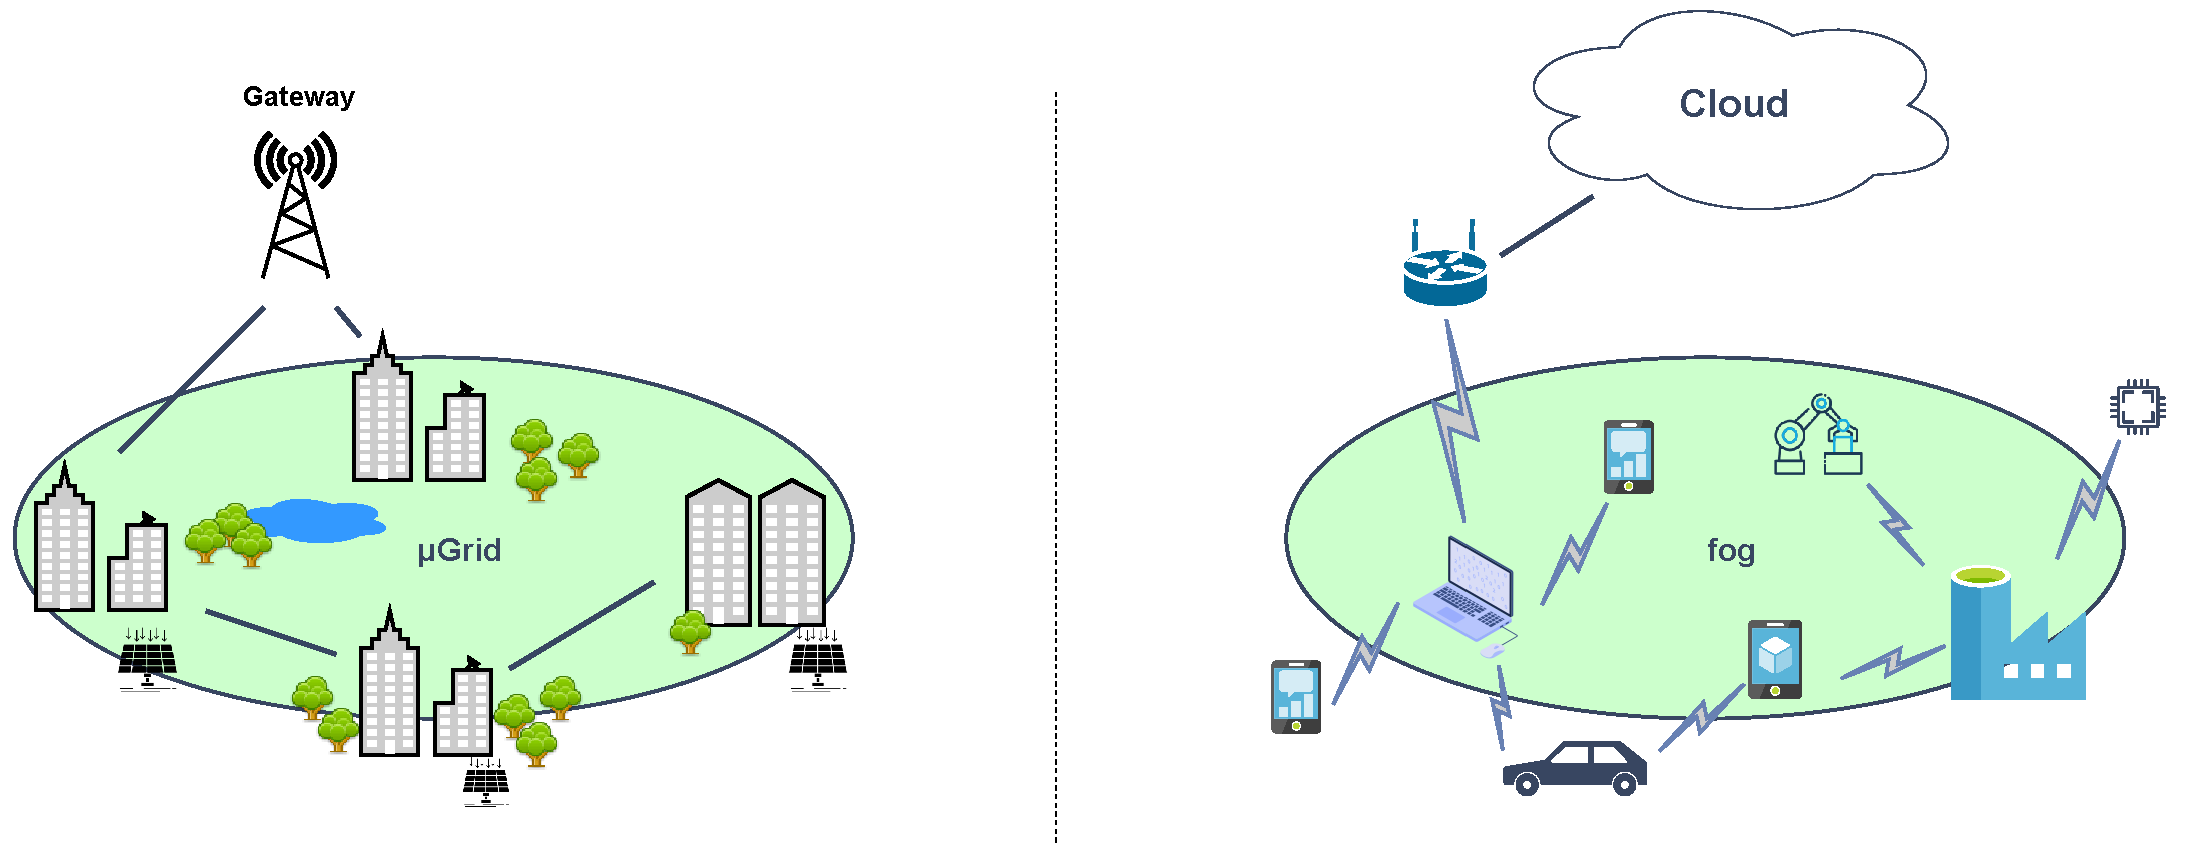
\includegraphics[width=\textwidth]{fig/05_den2ne/den2ne_01.drawio.pdf}
    \caption{Dos ejemplos de redes que aprovecharían DEN2NE para equilibrar los recursos.}
    \label{fig:den2ne_01}
\end{figure}

Estos sistemas necesitan redistribuir la producción excedente entre otros consumidores, y dicha distribución energética debe realizarse lo más cerca posible de la fuente para minimizar las pérdidas por transmisión. En la parte derecha se representa una red de \textit{fog computing}, compuesta por diversos dispositivos \gls{iot}, como ordenadores portátiles, teléfonos móviles, automóviles o robots industriales. En este último escenario, un nodo \gls{iot} podría necesitar ejecutar una tarea, y descargarla (hacer un \textit{offload}) entre otros dispositivos cercanos con recursos de cómputo disponibles podría acelerar su finalización. Como puede observarse, ambas implementaciones requieren algoritmos análogos para compartir una o varias acciones/tareas que deben completarse (por ejemplo, producción de energía, cómputo de una tarea, etc.). Además, ambos ejemplifican una porción de una red mucho mayor, lo que implica que disponen de una conexión (p. ej., un \textit{gateway}) con el resto de esa red global. Por ejemplo, una \textit{microgrid} podría usar el \textit{gateway} para enviar o recibir energía del resto del despliegue de la red inteligente, y lo mismo ocurre en el entorno \textit{fog}, que podría delegar la resolución de la tarea en la nube en el peor de los casos (es decir, cuando todos los nodos están saturados y no pueden procesarla localmente).\\
\\
En consecuencia, el objetivo principal de nuestro algoritmo es redistribuir de forma eficiente recursos entre cualquier tipo de nodos conectados. Para ello, cualquier nodo que actúe como fuente puede delegar un recurso a cualquier nodo destino. En este sentido, la formulación del problema se asemeja a un problema de encaminamiento (según se estudió en la Sección~\ref{subsubsec:conclu_recursos}), con una diferencia: en el encaminamiento hay una información que debe entregarse desde un origen concreto a un destino concreto y solo es necesario calcular la ruta; en este caso, aunque existe un origen y una información definida, los destinos potenciales pueden ser múltiples, y deben decidirse conjuntamente con la ruta que seguirá la información/recurso a distribuir. Dicho de otro modo, un recurso puede compartirse entre uno o varios nodos destino, y esa decisión debe calcularse por el algoritmo, junto con las rutas para alcanzarlos.\\
\\
Para cumplir el objetivo anterior, el diseño del \gls{d2e} se sustenta en tres principios fundamentales:

\begin{enumerate}

    \item \textbf{Tiempo de rápido convergencia}: la decisión sobre el reparto de recursos debe computarse con rapidez; es decir, el algoritmo debería presentar un tiempo de convergencia bajo. Además, dicho tiempo no debería verse penalizado de forma drástica por la cantidad de datos/recursos disponibles o por el número de nodos de la red; idealmente crecerá de manera cercana a lineal con el tamaño de la red ($\mathcal{O}(n)$). Tiempos de convergencia cortos facilitan actualizaciones ágiles en escenarios de alta movilidad.
    
    \item \textbf{Baja complejidad}: dado que los nodos que ejecutarán el algoritmo suelen ser dispositivos con recursos limitados (memoria, batería, CPU), el método debe exigir poca capacidad de cómputo y almacenamiento, e implicar un número reducido de mensajes de control intercambiados.
    
    \item \textbf{Versatilidad}: además de escalable, el algoritmo debe ser fácil de adaptar a distintos entornos prácticos (redes cableadas e inalámbricas, \gls{sg}, entornos \gls{iiot}, enfoques centralizados o distribuidos, etc.). En concreto, su diseño debe evitar supuestos demasiado restrictivos sobre la infraestructura, para permitir su reutilización en escenarios variados.
\end{enumerate}

Sobre la base de estos tres principios, se tomó como punto de partida el protocolo de encaminamiento IoTorii de Rojas \textit{et al.}~\cite{rojas2021outperforming} (Analizado en la Sección~\ref{subsubsec:propuestas_etiquetado}), ya que cumple con requisitos de convergencia rápida y bajo consumo de recursos. Aunque IoTorii está concebido como protocolo de encaminamiento, su naturaleza distribuida facilita transformarlo a una versión centralizada si fuera necesario. No obstante, dado que IoTorii selecciona rutas para pares origen–destino concretos, ha de adaptarse para satisfacer los objetivos del \gls{d2e}, que no asume un conjunto de destinos predefinidos de partida. En particular, el \gls{d2e} se diseña para localizar los vecinos más cercanos a los que se puede delegar una tarea o recurso. En este escenario se asume la existencia, de al menos, un nodo con acceso a recursos <<ilimitados>>, que actúe como sumidero de recursos de la red; a dicho nodo lo denominamos \textit{gateway} o nodo raíz (\textit{root}). Los \textit{gateway} pueden asumir la porción restante de la tarea o recurso cuando el \textit{offloading} local no sea factible. En las siguientes sub-Secciones se describirá en detalle el algoritmo \gls{d2e}.

\subsection{Terminología del algoritmo}
\label{subsec:terminologiaDEN2NE}
Una vez presentada la motivación del algoritmo y antes de profundizar en su descripción, definiremos algunos términos que se emplearán posteriormente. Para mayor claridad, nos centraremos en la Figura~\ref{fig:den2ne_02}, como ejemplo de escenario de aplicación. En dicho escenario, contamos con seis nodos (representados como círculos) conectados a un nodo raíz (\textit{root}). Los nodos están conectados bidireccionalmente (ya sea de forma cableada o inalámbrica), como indican las flechas negras bidireccionales más oscuras, y sus números simbolizan un <<recurso>> que debe ser distribuido o balanceado. Más concretamente, dicho recurso puede representar una \textbf{oferta} o una \textbf{demanda} (por ejemplo, producción/consumo eléctrico o capacidades computacionales disponibles o requeridas). En el caso de la Figura~\ref{fig:den2ne_02}, los valores negativos expresan una demanda, mientras que los positivos expresan una oferta. En este sentido, por ejemplo, una demanda de -80 se compensaría con una oferta equivalente de +80 o, alternativamente, con una combinación de ofertas que sumaran +80. Por lo tanto, el objetivo principal de nuestro algoritmo es compensar todos los recursos en la red, es decir, que todos los nodos tiendan hacia el valor cero (un uso óptimo), mientras que el remanente (ya sea exceso de demanda u oferta) se redirija hacia el nodo raíz. \\
\\
Antes de describir las tres fases del algoritmo \gls{d2e} (en las Secciones~\ref{subsec:fase1}, \ref{subsec:fase2}, y \ref{subsec:fase3}, respectivamente), reflexionemos sobre el ejemplo de la Figura~\ref{fig:den2ne_02} para entender por qué se definieron tres fases. Considerando los principios de diseño mencionados anteriormente, calcular todas las posibles combinaciones de reparto no es factible en un tiempo razonable. Por otro lado, la información local podría reducir los tiempos de convergencia y la complejidad, pero tampoco sería suficiente para decidir de manera óptima. Como ejemplo de una mala decisión, el nodo con una demanda de -80 solo conoce a sus dos vecinos: uno que ofrece (+100) y otro que demanda (-10), y podría pensar que el nodo más adecuado para cubrir su demanda (-80) es el vecino inferior (+100) (en la Figura~\ref{fig:den2ne_02}). Sin embargo, esta decisión local resulta ser incorrecta, ya que existen otros nodos con demandas adicionales (-50, -40 y -30), que también requieren de esa oferta y se encuentran mucho más alejados del nodo raíz. De hecho, la solución de distribución óptima se ilustra con flechas naranjas claras (que representan la dirección desde el nodo demandante hacia el nodo con oferta). Esta distribución implicaría que todos los nodos quedaran balanceados en cero y que la demanda restante de -110 (suma de -50 -40 -30 +100 -80 -10) se desviara hacia el nodo raíz, el cual, sería capaz de cubrirla.


\begin{figure}[ht!]
    \centering
    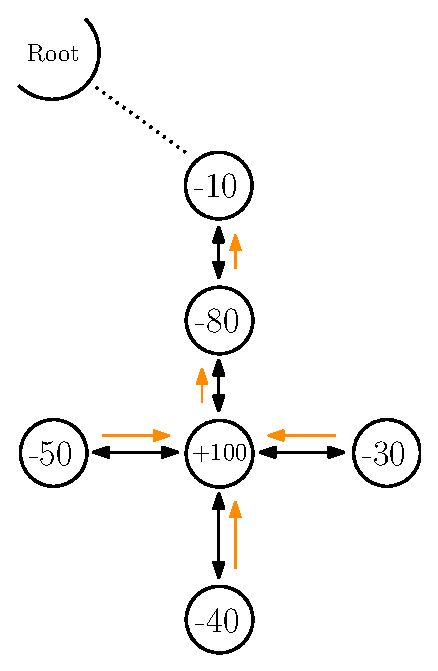
\includegraphics[width=0.4\textwidth]{fig/05_den2ne/den2ne_02.eps}
    \caption{Ejemplo de equilibrio de recursos en una red con seis nodos y un \textit{gateway} (o nodo raíz).}
    \label{fig:den2ne_02}
\end{figure}

Consecuentemente, el algoritmo \gls{d2e} calcula la distribución de recursos considerando información de todos los nodos atravesados, en lugar de limitarse únicamente a la información local de los vecinos. Además, prioriza la distribución en los nodos más alejados del nodo raíz, arrastrando el remanente (oferta o demanda) hacia la raíz para que pueda ser compensado allí por el resto de la red (por ejemplo, la nube o la \textit{smartgrid}).\\
\\
En las subsecciones siguientes se describen en detalle las tres fases que componen el algoritmo. La primera fase está dedicada a explorar la topología y agregar información de los nodos recorridos mediante etiquetado jerárquico; la segunda selecciona, entre todas las etiquetas recibidas, el conjunto de información que parece más cercano a la solución óptima; y la tercera ejecuta el balance de recursos en función de la decisión tomada en la fase segunda. Más concretamente:

\begin{itemize}
    \item En la \textbf{Fase 1} (Subsección~\ref{subsec:fase1}) se explica el etiquetado jerárquico para calcular rutas desde cada nodo hasta el nodo raíz. Esta fase se inspira en los trabajos relacionados sobre encaminamiento escalable y resiliente examinados en la Sección~\ref{subsubsec:propuestas_etiquetado}.
    
    \item En la \textbf{Fase 2} (Subsección~\ref{subsec:fase2}), una vez que se han generado todas las rutas posibles hacia la raíz, se selecciona, en cada nodo, una de ellas siguiendo un criterio concreto. Este criterio proporciona la versatilidad prevista como principio de diseño: proponemos seis criterios para que el más adecuado se aplique según el escenario, aunque en la práctica cualquier otro criterio nuevo podría emplearse si fuese necesario.
    
    \item En la \textbf{Fase 3} (Subsección~\ref{subsec:fase3}), tras la selección de la ruta activa ($ID_{activa}$) en la fase anterior, se realiza el balanceo de recursos en base a la lista de nodos representada por las etiquetas activas. Esta fase tiene en cuenta además las condiciones reales de la red, por ejemplo, si los enlaces presentan pérdidas o capacidades limitadas.
\end{itemize}


\subsection{Fase 1 - Etiquetado jerárquico}
\label{subsec:fase1}

El algoritmo \gls{d2e} comienza localizando las posiciones relativas de cada nodo en la red. Para ello, se realiza un etiquetado jerárquico a partir de cada nodo raíz presente en el despliegue. Como algoritmo centralizado, cada nodo dispone de un identificador numérico único (ID) que les identifica en la red, y obtienen durante el proceso una etiqueta jerárquica que les indicará su posición en la topología, y una ruta para alcanzar el sumidero de la misma. Este mecanismo de etiquetado jerárquico comparte ciertos aspectos con el descrito en el Capítulo~\ref{ch:propuestaInband}, sin embargo, en vez de emplear un etiquetado basado en sufijos auto-asignados en procesos de reconocimiento de vecindad, se emplearán identificadores únicos, aligerando el proceso de exploración de la topología. La Figura~\ref{fig:den2ne_03} presenta el esquema de etiquetado diseñado. 


\begin{figure}[ht!]
    \centering
    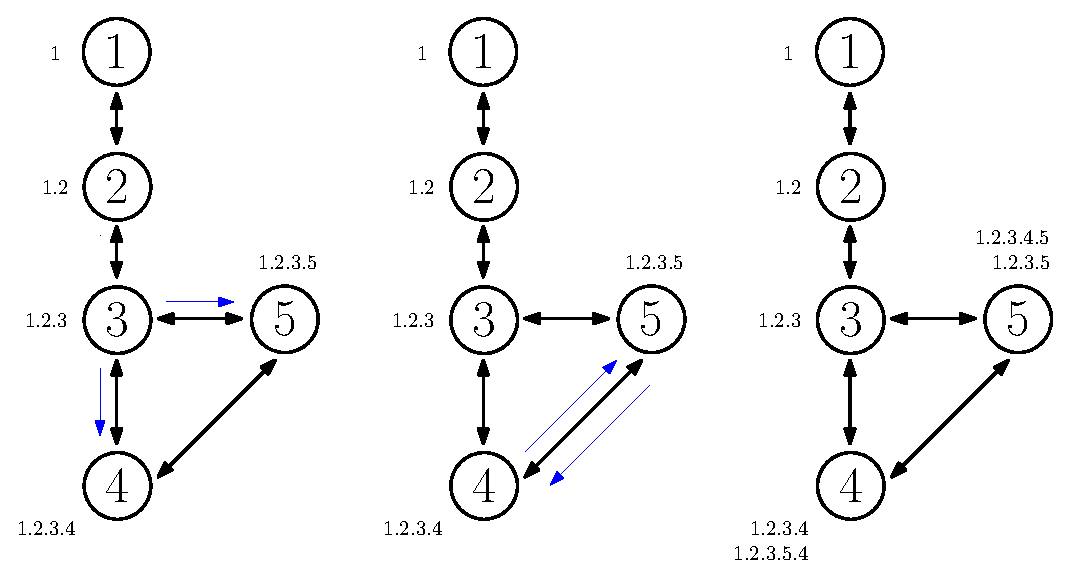
\includegraphics[width=0.9\textwidth]{fig/05_den2ne/den2ne_03.eps}
    \caption{Procedimiento de etiquetado jerárquico en DEN2NE.}
    \label{fig:den2ne_03}
\end{figure}

El procedimiento parte en el nodo raíz, que en la Figura~\ref{fig:den2ne_03} tiene ID~1 y un vecino conectado con ID~2. Para correlacionarlos jerárquicamente, el algoritmo asigna la etiqueta \texttt{1} al raíz y concatena el ID del vecino a la suya propia, de modo que el nodo~2 recibe la etiqueta \texttt{1.2}. A continuación, el nodo con ID~3 obtendrá la etiqueta \texttt{1.2.3}, y los nodos con IDs~4 y~5 recibirán las etiquetas \texttt{1.2.3.4} y \texttt{1.2.3.5}, respectivamente. Además, conforme progresa la asignación, el nodo con ID~4 también podrá registrar la etiqueta \texttt{1.2.3.5.4} y el nodo con ID~5 la etiqueta \texttt{1.2.3.4.5}, según correspondan las rutas alternativas. Este procedimiento de etiquetado continúa hasta que se explora toda la red y cada nodo dispone, al menos, de una etiqueta jerárquica. En la práctica, cada etiqueta representa una ruta para alcanzar el nodo raíz, por lo que, nodos con múltiples rutas tendrán capacidad de balancear sus recursos por rutas alternativas.\\
\\
Para evitar bucles durante la fase de etiquetado jerárquico, el algoritmo no asigna a un nodo etiquetas que lo hereden de sí mismo. Esto se puede prever fácilmente ya que las etiquetas concatenan los IDs de los nodos recorridos, por lo que ninguna etiqueta debe contener un mismo ID repetido; de lo contrario, indicaría la existencia de un bucle en la ruta. Por ejemplo, la Figura~\ref{fig:den2ne_04} ilustra gráficamente esta restricción y muestra el siguiente paso respecto a lo representado en la Figura~\ref{fig:den2ne_03}. Cuando el nodo con ID~4 recibe la etiqueta \texttt{1.2.3.5.4} del nodo con ID~5, podría intentar propagar la etiqueta \texttt{1.2.3.5.4.3} hacia el nodo con ID~3, pero esta acción no se realiza porque la etiqueta contiene el ID~3 en dos ocasiones, lo que representaría un bucle. Una vez descartada dicha etiqueta, no se propagarán más etiquetas que la deriven. De manera análoga, si el nodo con ID~5 generara \texttt{1.2.3.4.5.3} para el nodo~3, esta también sería rechazada por el mismo motivo. En este ejemplo concreto, tras estos pasos descritos, no se asignan más etiquetas y el procedimiento del etiquetado jerárquico habría concluido en este punto.


\begin{figure}[ht!]
    \centering
    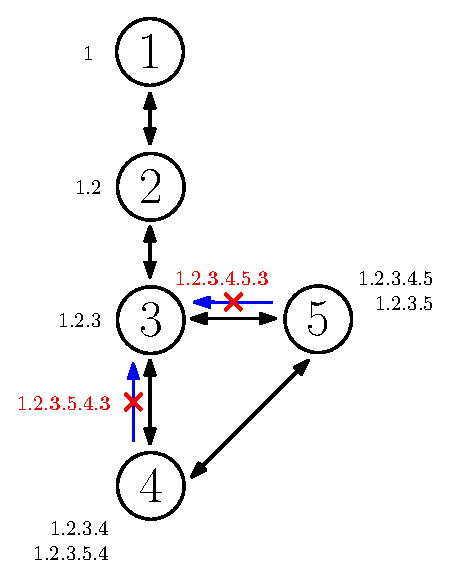
\includegraphics[width=0.4\textwidth]{fig/05_den2ne/den2ne_04.eps}
    \caption{Mecanismo de evitación de bucles durante el etiquetado jerárquico.}
    \label{fig:den2ne_04}
\end{figure}

Como se indicó anteriormente, cada etiqueta asignada representa una ruta hacia la raíz y cada nodo obtiene una o varias etiquetas (es decir, múltiples rutas hacia el nodo raíz). Por tanto, esta primera fase del algoritmo puede calcular, en principio, todas las rutas posibles desde cualquier nodo de la red hasta la raíz. Esto puede conllevar miles o incluso millones de rutas, según la conectividad de la topología. Por ello, desde el punto de vista de la implementación, la fase de etiquetado jerárquico suele limitarse a aprender únicamente un subconjunto de etiquetas y descartar el resto siguiendo ciertos parámetros, como la disjunción de rutas o un número mínimo de saltos~\cite{Lopez-Pajares19}. El Algoritmo~\ref{alg:labeling} resume todo el procedimiento de la Fase 1, el cual, toma como entrada el grafo de la red y el nodo desde el que se inicia el etiquetado jerárquico (es decir, el nodo raíz) y devuelve el grafo con la asignación de etiquetas correspondiente. El algoritmo recorre los nodos partiendo de los vecinos del nodo raíz. Un nodo puede ser procesado más de una vez, hasta un máximo de etiquetas asignadas (\(\textup{IDs\_MAX}\)) o hasta que se detecte un bucle (\(\textit{check\_loop()}\)). Por este motivo, podemos afirmar que la complejidad de la fase de etiquetado es \(\mathcal{O}(n)\), ya que crece de forma lineal con el número de nodos \(n\), cada uno visitado como máximo \(\textup{IDs\_MAX}\) veces; dado que \(\textup{IDs\_MAX}\) se considera una constante de diseño, la complejidad asintótica se mantiene en \(\mathcal{O}(n)\) independientemente de la forma o tamaño de la topología.


\begin{algorithm}[ht!]
\caption{Proceso de etiquetado jerárquico}\label{alg:labeling}
\SetKwInOut{Input}{input}
\SetKwInOut{Output}{output}
\Input{$\: G(\mathcal{N}, \mathcal{L}),\: root$}
\Output{$\: G(\mathcal{N}, \mathcal{L})$}
\vspace{0.2cm}
$\textup{init}\: nodes\_to\_attend$\;
$\mathcal{N}(root).push(\texttt{ID}(\textup{None}, root))$\;
$nodes\_to\_attend.push(\mathcal{N}(root))$\;
\vspace{0.2cm}
\While{$length(nodes\_to\_attend) > \emptyset$}{
\vspace{0.1cm}
$curr\_node \: = \: nodes\_to\_attend[0]$\;
\vspace{0.1cm}  
\For{$j \: \gets \: length(curr\_node.ids)$}{
    \vspace{0.1cm}  
    \uIf{$not \: curr\_node.ids[j].used$}{
        \vspace{0.1cm}  
        \For{$neighbor \: \gets \: curr\_node.neighbors$}{
            \vspace{0.1cm}
            \uIf{$check\_loop(curr\_node.ids[j], neighbor)$}{
                $\textup{pass}$\;
            }
            \uElseIf{$neighbor.ids \:  \geq \textup{IDs\_MAX}$}{
                $\textup{pass}$\;
            }
            \Else{
                $\mathcal{N}(neighbor).push(\texttt{ID}(curr\_node.ids[j], neighbor))$\;
            }
            \vspace{0.1cm}
            $nodes\_to\_attend.push(\mathcal{N}(neighbor))$\;
        }
        \vspace{0.1cm}
        $curr\_node.ids[j].used \: = \: \textup{true}$\;
    }
}

  $pop\: nodes\_to\_attend[0]$\;
  
}
\vspace{0.1cm}
\Return{$G(\mathcal{N}, \mathcal{L})$}
\end{algorithm}


\subsection{Fase 2 - Selección de las mejores etiquetas o identificadores jerárquicos}
\label{subsec:fase2}

Como se ha presentado anteriormente, los nodos raíz o \textit{gateways} son aquellos conectados a recursos externos (energía, capacidad de cómputo, etc.) que pueden considerarse prácticamente <<ilimitados>>. Por este motivo, al repartir una tarea o recurso, los nodos más alejados del nodo raíz tienen menor probabilidad de disponer de recursos locales, mientras que los nodos próximos a la raíz pueden delegar con facilidad en el \textit{gateway} para completar la operación. La primera fase del algoritmo aporta precisamente la localización relativa de los nodos respecto a la raíz/raíces, lo que permite priorizar de forma natural qué nodos deben considerarse preferentes a la hora de decidir dónde delegar una tarea; en suma, simplifica y ordena el proceso de toma de decisiones.\\
\\
Concretamente, una vez finalizado el etiquetado jerárquico, cada nodo dispone de una o varias etiquetas que representan rutas hacia la raíz, dado que cada etiqueta codifica la lista de nodos a atravesar para alcanzarla. Si un nodo cuenta con una única etiqueta, existe un único camino conocido hacia la raíz; si dispone de varias, hace falta aplicar criterios de selección para escoger la ruta más adecuada. Dado que las rutas hacia la raíz se construyen de forma coordinada entre nodos, ese criterio de selección debe aplicarse respetando un cierto orden y coordinación entre los participantes.\\
\\
La segunda fase del algoritmo, por tanto, decide dónde distribuir los recursos aplicando criterios sobre las etiquetas o identificadores jerárquicos obtenidos en la primera fase. Como referencia, el algoritmo \gls{d2e} incorpora seis criterios distintos (basados en la literatura) para puntuar cada ruta disponible: cada criterio calcula un coste asociado a una etiqueta concreta (denotado $Cost_{ID}$). A continuación, se selecciona la ruta activa, el identificador jerárquico activo $ID_{activa}$, como la que minimiza dicho coste, tal y como se expresa en la Ecuación~\ref{eq:IDactiveCost}.

\begin{align}\label{eq:IDactiveCost}
     \left \langle ID_{activa} \right \rangle  \: &  = \: min(Cost_{ID})
\end{align}

Los seis criterios se describen en las secciones siguientes. Es importante remarcar que pueden definirse e incorporar criterios adicionales al algoritmo: la segunda fase únicamente exige la especificación de una función de coste para cada criterio, por lo que la elección concreta no limita el funcionamiento del método y, de hecho, dota de versatilidad a la propuesta. Asimismo, algunos criterios resultan aplicables de forma genérica a múltiples casos de uso, mientras que otros son específicos de dominios concretos (p. ej. \gls{sg}, \textit{fog computing}, etc.). Por estas razones, los criterios se presentan de forma concisa y directa a modo de referencia; en la práctica, \gls{d2e} es potencialmente agnóstico respecto al criterio seleccionado.

\subsubsection{Criterio 1 - Número de saltos}

Este primer criterio evalúa el número de saltos necesarios para alcanzar el nodo raíz, de modo que en cada nodo se selecciona el identificador jerárquico con menor número de saltos. Se basa en el clásico criterio de camino más corto para encaminamiento en redes de comunicaciones, denominado \emph{widest-shortest path}, Ma \textit{et al.}~\cite{Ma97}. Por tanto, la función de coste para este criterio puede expresarse como en la Ecuación~\ref{eq:criterionCost01}. 

\begin{equation}\label{eq:criterionCost01}
     Cost_{ID}  \: = \: length(ID) \: - \: 1
\end{equation}
\vspace{0.2cm}

Para comprenderlo, la Figura~\ref{fig:den2ne_05} muestra un ejemplo en el que el nodo 5 ha adquirido tres identificadores jerárquicos y se representan las tres rutas potenciales hacia la raíz (nodo 1). En este escenario, el coste se calcula como la longitud del identificador (donde la longitud es el número de cifras en la etiqueta jerárquica) menos uno; por ejemplo, para el identificador \texttt{1.2.3.5} el coste es $3 = 4 - 1$, dado que dicho identificador tiene 4 cifras. Una vez calculado el coste para cada identificador jerárquico, el identificador seleccionado en el ejemplo es \texttt{1.2.3.5} conforme a la Ecuación~\ref{eq:IDactiveCost}, pues presenta el menor coste, lo que implica menos saltos para alcanzar la raíz. En caso de fallo o indisponibilidad de esa ruta principal, cualquiera de las rutas restantes podría emplearse, ordenadas por coste. 

\begin{figure}[ht!]
    \centering
    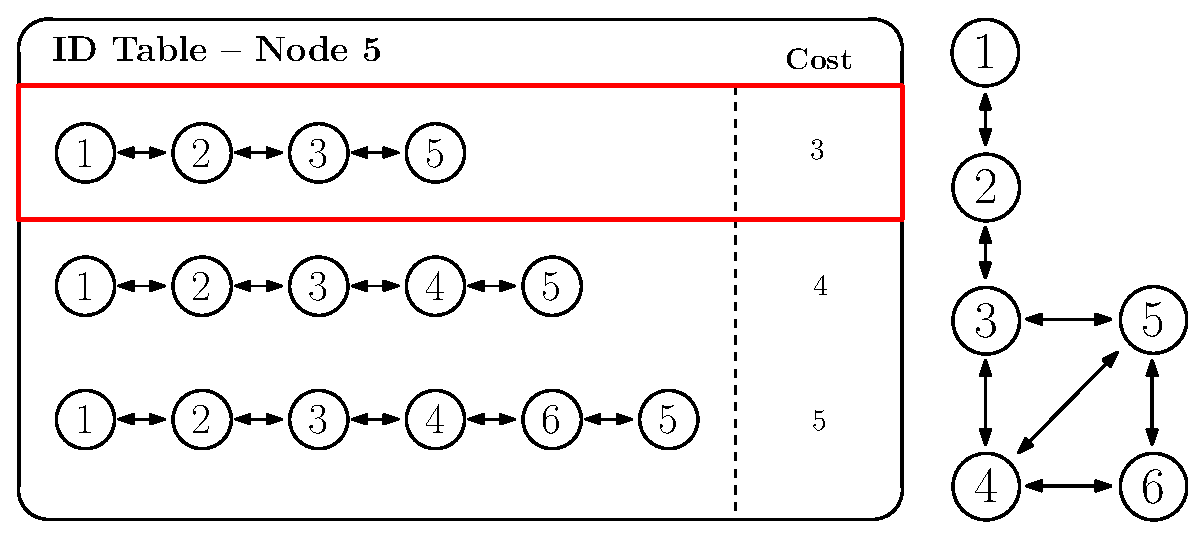
\includegraphics[width=0.9\textwidth]{fig/05_den2ne/den2ne_05.eps}
    \caption{Selección de ID basada en el criterio del número de saltos.}
    \label{fig:den2ne_05}
\end{figure}


\subsubsection{Criterio 2 - Distancia}

El segundo criterio incorpora el concepto de distancia entre nodos. Dicha distancia puede ser física (por ejemplo, en despliegues de \textit{microgrids}, donde la distancia física es conocida y constante porque los nodos no son móviles) o lógica (por ejemplo, un coste de enlace basado en el rendimiento o la latencia en un despliegue de red). Al igual que el criterio anterior, se inspira en técnicas clásicas de encaminamiento en redes de comunicaciones y recibe el nombre de \textit{shortest-distance path}, Ma \textit{et al.}~\cite{Ma97}. En este caso, el coste de cada identificador jerárquico se calcula como la suma de las distancias de los enlaces recorridos, tal como se expresa en la Ecuación~\ref{eq:criterionCost02} (una ``distancia'' puede equivaler también al inverso del \textit{throughput} del enlace u otra métrica relacionada).

\begin{equation}\label{eq:criterionCost02}
     Cost_{ID}  \: = \: \sum_{i=0}^{N_{saltos}-1} d_{i}
\end{equation}
\vspace{0.2cm}

La Figura~\ref{fig:den2ne_06} muestra el mismo ejemplo anterior aplicado con este segundo criterio. En dicho escenario, el identificador \texttt{1.2.3.5} resulta seleccionado si se cumple la condición indicada en la Ecuación~\ref{eq:criterionCost02_b}; no obstante, dependiendo de los valores reales de las distancias, podría seleccionarse cualquier otro identificador aunque la ruta tenga más saltos hasta la raíz.

\begin{equation}\label{eq:criterionCost02_b}
     \left \langle ID_{1} = ID_{activa} \right \rangle \Leftrightarrow 
     \left\{\begin{matrix}
      [d_{35} < ( d_{34} + d_{45})] \\
      \\
       \wedge \\ 
       \\
      [d_{35} < ( d_{34} + d_{46} + d_{65})] 
      \end{matrix}\right.
\end{equation}
\vspace{0.2cm}

\begin{figure}[ht!]
    \centering
    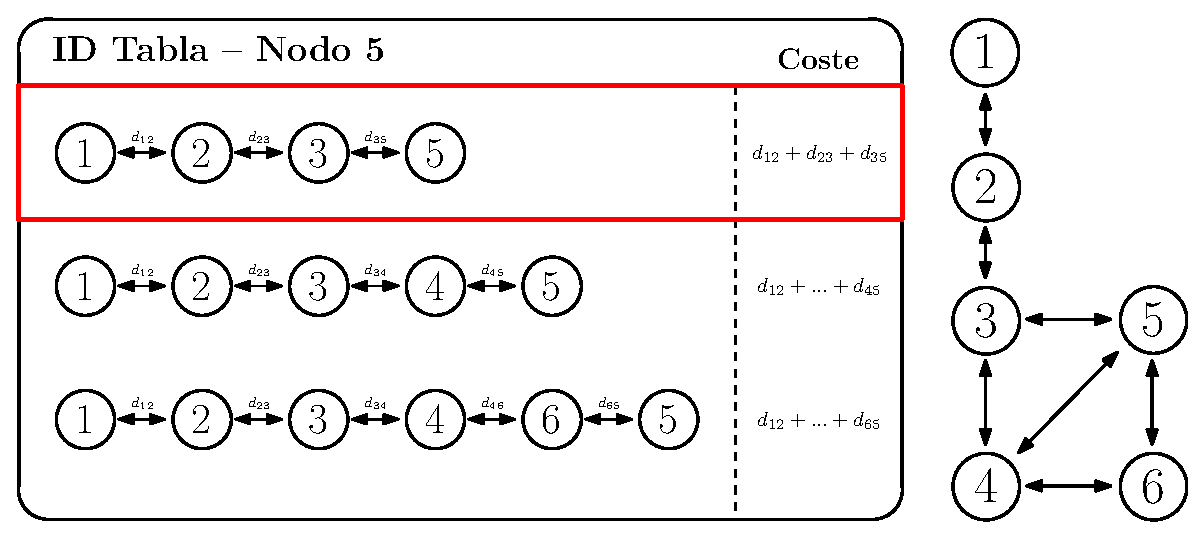
\includegraphics[width=0.9\textwidth]{fig/05_den2ne/den2ne_06.eps}
    \caption{Selección de ID basada en el criterio de distancia.}
    \label{fig:den2ne_06}
\end{figure}

\subsubsection{Criterio 3 - Pérdidas de enlace}

El tercer criterio está directamente relacionado con el caso de uso de redes inteligentes de distribución eléctrica (inspirado en la topología IEEE 123-node test feeder~\cite{Schneider17}) en el que puede aplicarse este algoritmo, y se vincula asimismo con el criterio anterior sobre distancia. Concretamente, se persigue la minimización de las pérdidas en los enlaces debidas a la transmisión. Para distinguirlo del criterio 2, conviene subrayar que el criterio 2 suele centrarse en características del enlace o su capacidad (p. ej. rendimiento o distancia), mientras que el criterio 3 atiende al efecto de degradación del enlace (p. ej. pérdidas de potencia). No obstante, ambos criterios están estrechamente relacionados y, de hecho, su formulación es conceptualmente similar, intercambiando distancias por pérdidas, como se muestra en la Ecuación~\ref{eq:criterionCost05}.

\begin{equation}\label{eq:criterionCost05}
      Cost_{ID}  \: = \: \sum_{ij}^{N_{ID}} L_{ij} \: = \: \sum_{ij}^{N_{ID}} (\frac{\alpha_{R_{ij}} \: \times \: d_{ij}}{V_{d}^{2}}\: \times \: P_{in}^{2})
\end{equation}
\vspace{0.2cm}

En el caso específico de las redes eléctricas, las pérdidas se calculan a partir de modelos de pérdidas en líneas de transmisión que consideran parámetros tales como: tensión ($V_{d}$), distancia física ($d_{ij}$), coeficiente de reflexión ($\alpha_{R_{ij}}$) y potencia de entrada ($P_{in}$), tal y como recoge la Ecuación~\ref{eq:criterionCost04_b} (incorporada en la Ecuación~\ref{eq:criterionCost05}). Como puede apreciarse, la distancia física es uno de los parámetros que afectan al coste, pero no el único. Por ello, como hemos mencionado antes, los criterios 2 y 3 están relacionados pero no necesariamente producen el mismo resultado, pues intervienen factores adicionales. En otros escenarios, las ``pérdidas'' podrían interpretarse de forma análoga (p. ej. fiabilidad de enlace en un entorno inalámbrico para computación).

\begin{equation}\label{eq:criterionCost04_b}
     L_{ij} \: = \: \frac{\alpha_{R_{ij}} \: \times \: d_{ij}}{V_{d}^{2}}\: \times \: P_{in}^{2}
\end{equation}
\vspace{0.2cm}

En el ejemplo concreto de la Figura~\ref{fig:den2ne_07}, la ruta hacia el nodo raíz seleccionada como $ID_{activa}$ es la primera (\texttt{1.2.3.5}), que en este caso coincide con la escogida por el criterio anterior. Siempre y cuando, la condición indicada en la Ecuación~\ref{eq:criterionCost05_b} se cumpla. 

\begin{equation}\label{eq:criterionCost05_b}
       \left \langle ID_{1} = ID_{active} \right \rangle \Leftrightarrow 
       \left\{\begin{matrix}
       [\sum_{\substack{1 \leq i \leq 3\\ 2 \leq j \leq 5\\ j \neq 4}}^{} L_{ij} < \sum_{\substack{1 \leq i \leq 4 \\  2 \leq j \leq 5}}^{} L_{ij}]\\
       \\
       \wedge \\ 
       \\
       [\sum_{\substack{1 \leq i \leq 3\\ 2 \leq j \leq 5\\ j \neq 4}}^{} L_{ij} < \sum_{\substack{1 \leq i \leq 5 \\ 2 \leq j \leq 6}}^{} L_{ij}]
       \end{matrix}\right.
\end{equation}
\vspace{0.2cm}

\begin{figure}[ht!]
    \centering
    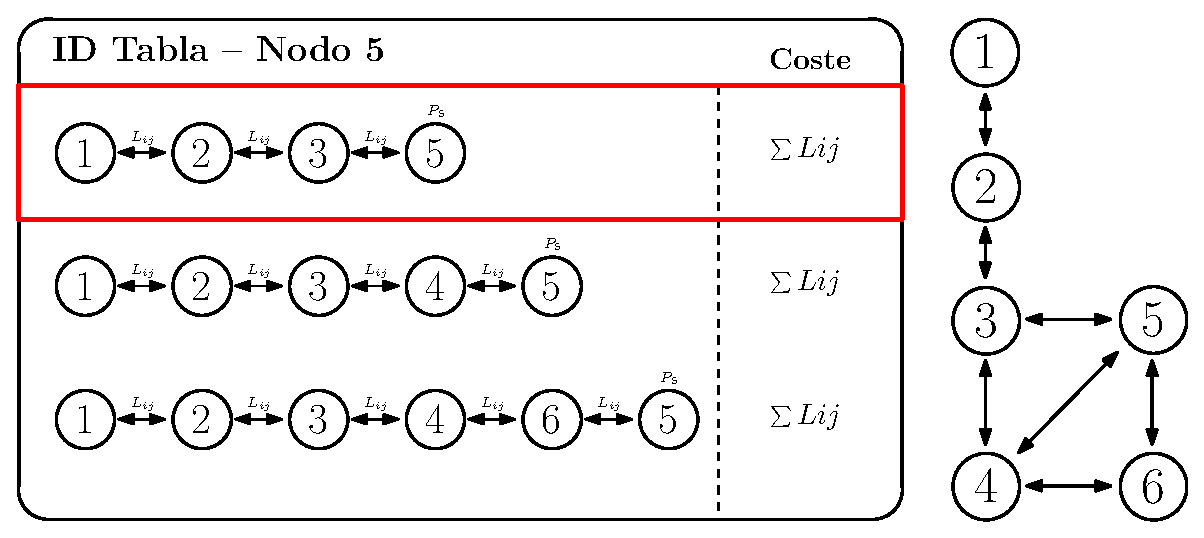
\includegraphics[width=0.9\textwidth]{fig/05_den2ne/den2ne_07.eps}
    \caption{Selección de ID basada en el criterio de pérdidas de enlace.}
    \label{fig:den2ne_07}
\end{figure}

\subsubsection{Criterio 4 - Balance de potencia}

El cuarto criterio evalúa las rutas con más recursos disponibles en su recorrido, y las selecciona preferentemente frente a otras. Dado que cada nodo puede tener una oferta de recursos (valor positivo) o una demanda (valor negativo), la suma de todos los valores a lo largo de la ruta representará un coste total de la misma, tal y como se define en la Ecuación~\ref{eq:criterionCost03}. Este coste se calcula cambiando el signo de la suma de todas las potencias en el trayecto, ya que nuestro objetivo es minimizarlo. Por lo tanto, si existen muchas ofertas de recursos, la suma será un valor positivo elevado y, al invertir su signo, se traducirá en un valor muy negativo (es decir, un bajo coste). Es importante destacar que el nombre de este criterio proviene del caso de uso de las redes eléctricas inteligentes, en el que los recursos son la potencia eléctrica. Sin embargo, aunque en la fórmula se considere la oferta y la demanda de potencia, otros parámetros, como la capacidad de cómputo en entornos de \gls{cec}, podrían aplicarse de manera análoga en este criterio.  De hecho, en el campo del enrutamiento clásico, Ma~\textit{et al.}~\cite{Ma97} lo denominan \textit{shortest-widest path}.
\begin{equation}\label{eq:criterionCost03}
     Cost_{ID}  \: = \: -(\sum_{i}^{N_{ID}} P_{i})
\end{equation}

Una vez más, la selección de $ID_{activa}$ se basará en el valor mínimo de $Cost_{ID}$. En el caso de nuestro ejemplo, como se observa en la Figura~\ref{fig:den2ne_08}, el ID seleccionado es \texttt{1.2.3.4.6.5}, el cual debería cumplir con la condición de la Ecuación~\ref{eq:criterionCost03_b}.

\begin{equation}\label{eq:criterionCost03_b}
\begin{split}
     \left \langle ID_{3} = ID_{activa} \right \rangle \Leftrightarrow
     \left\{\begin{matrix}
     [\sum_{i}^{6}P_{i} > \sum_{i}^{5}P_{i}]\\
       \\
       \wedge \\ 
       \\
       [\sum_{i}^{6}P_{i} > \sum_{i,i\neq 4}^{5}P_{i}]
     \end{matrix}\right.
\end{split}
\end{equation}
\begin{figure}[ht!]
    \centering
    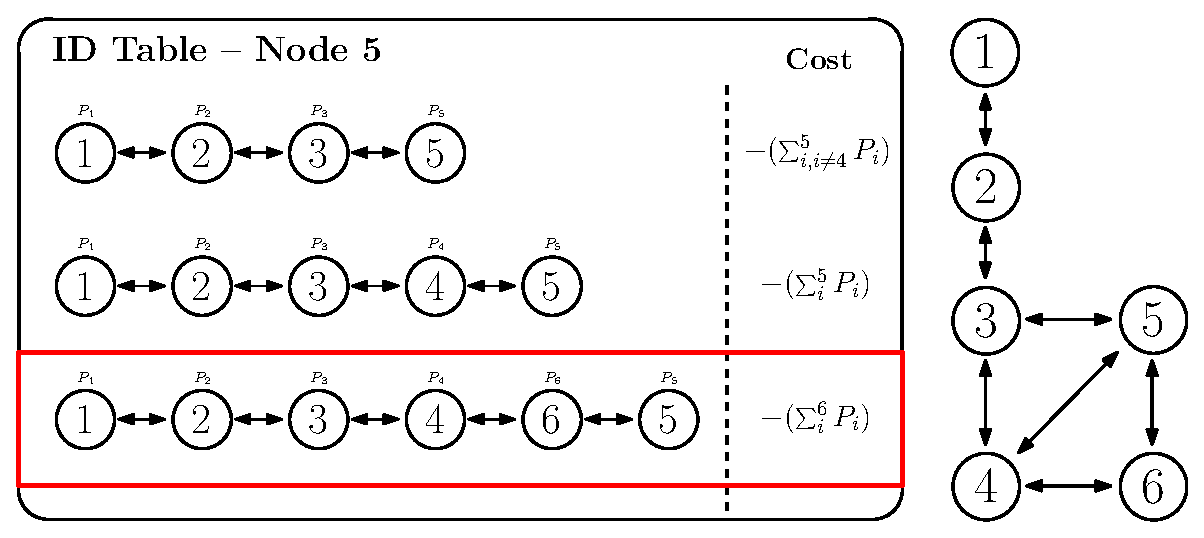
\includegraphics[width=0.9\textwidth]{fig/05_den2ne/den2ne_08.eps}
    \caption{Selección de ID basada en el criterio de balance de potencia.}
    \label{fig:den2ne_08}
\end{figure}

\subsubsection{Criterio 5 - Balance de potencia con pérdidas}

El quinto criterio combina los criterios 3 y 4~\cite{Schneider17,Ma97}, ya que busca maximizar los recursos disponibles en la ruta, al mismo tiempo que limita las pérdidas potenciales que una ruta específica (especialmente si es más larga que otras), pueda conllevar. Una vez más, en el caso de las redes eléctricas inteligentes, esto se traduce en la oferta y la demanda de potencia, restando las pérdidas en la ruta (que siguen la Ecuación~\ref{eq:criterionCost04_b}), tal y como se representa en la Ecuación~\ref{eq:criterionCost04}.  
 

\begin{equation}\label{eq:criterionCost04}
     Cost_{ID}  \: = \: -(\sum_{i}^{N_{ID}} P_{i} - \sum_{ij}^{N_{ID}-1} L_{ij})
\end{equation}
\vspace{0.2cm}

Cuando este criterio se aplica al ejemplo de la Figura~\ref{fig:den2ne_09}, la ruta seleccionada es \texttt{1.2.3.4.5}, que en realidad representa una decisión intermedia entre el criterio 3 (pérdidas en los enlaces) y el criterio 4 (balance de potencia). En consecuencia, debe cumplirse la condición de la Ecuación~\ref{eq:criterionCost04_c} para que el $ID_{activa}$ corresponda al mostrado en la Figura~\ref{fig:den2ne_09}.


\begin{equation}\label{eq:criterionCost04_c}
\begin{split}
     \left \langle ID_{2} = ID_{activa} \right \rangle \Leftrightarrow 
     \left\{\begin{matrix}
    {\scriptstyle [(\sum_{i}^{6}P_{i} - \sum L_{ij} ) > (\sum_{i}^{5}P_{i} -  \sum L_{ij})]} \\
       \\
       \wedge \\ 
       \\
       {\scriptstyle[(\sum_{i}^{6}P_{i} -  \sum L_{ij}) > (\sum_{i,i\neq 4}^{5}P_{i} -  \sum L_{ij})]}
       \end{matrix}\right.
\end{split}
\end{equation}
\vspace{0.2cm}


\begin{figure}[ht!]
    \centering
    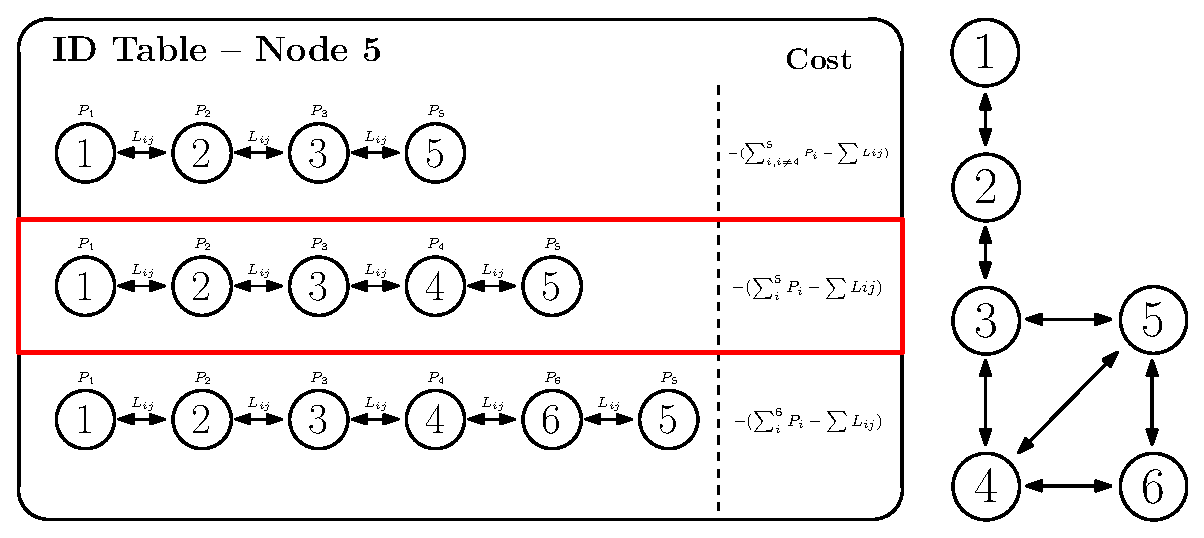
\includegraphics[width=0.9\textwidth]{fig/05_den2ne/den2ne_09.eps}
    \caption{Selección de ID basada en el criterio de balance de potencia con pérdidas.}
    \label{fig:den2ne_09}
\end{figure}

\subsubsection{Criterio 6 - Balance de potencia ponderado}

El sexto y último criterio representa una implementación alternativa, mediante ponderaciones, de las ideas presentadas en los dos criterios anteriores~\cite{Schneider17,Ma97}. Mientras que el criterio 5 penaliza la ruta en función de la longitud y otros parámetros de pérdidas, el criterio 6 normaliza la capacidad de potencia de la ruta en función del número de nodos atravesados. Este criterio pone de manifiesto directamente el efecto negativo que puede tener el criterio 4, que busca el mayor balance de potencia, ya que eventualmente podría favorecer rutas más largas hacia la raíz. Por lo tanto, el criterio 5 reajusta este cálculo considerando también las pérdidas potenciales, y el criterio 6 proporciona un balance de potencia ponderado, de modo que se tenga en cuenta tanto la capacidad como el número de saltos en la ruta. Este criterio puede resultar particularmente útil cuando no se dispone de una representación clara de las pérdidas de los enlaces. La fórmula resultante se representa en la Ecuación~\ref{eq:criterionCost06}.  
 

\begin{equation}\label{eq:criterionCost06}
      Cost_{ID}  \: = \: -(\frac{1}{M}\sum_{i}^{N_{ID}} P_{i}), \: \: M = \frac{1}{(lenght(ID) \: - \: 1)}
\end{equation}
\vspace{0.2cm}

Considerando el ejemplo de la Figura~\ref{fig:den2ne_10}, el $ID_{activa}$ corresponde a la ruta \texttt{1.2.3.4.5}, que tiene un menor número de nodos que la seleccionada en el criterio 4, como era de esperar, pero presenta la mejor relación $\frac{recursos}{saltos}$ entre todas las rutas. Esta ruta cumple la condición representada en la Ecuación~\ref{eq:criterionCost06_b}.

\begin{equation}\label{eq:criterionCost06_b}
           \left \langle ID_{2} = ID_{activa} \right \rangle \Leftrightarrow  
           \left\{\begin{matrix}
           [\frac{1}{4}\sum_{i}^{5} P_{i} > \frac{1}{3}\sum_{i,i\neq4}^{5} P_{i}] \\
       \\
       \wedge \\ 
       \\ [\frac{1}{4}\sum_{i}^{5} P_{i} > \frac{1}{5}\sum_{i}^{6} P_{i}]
           \end{matrix}\right.
\end{equation}
\vspace{0.2cm}

\begin{figure}[ht!]
    \centering
    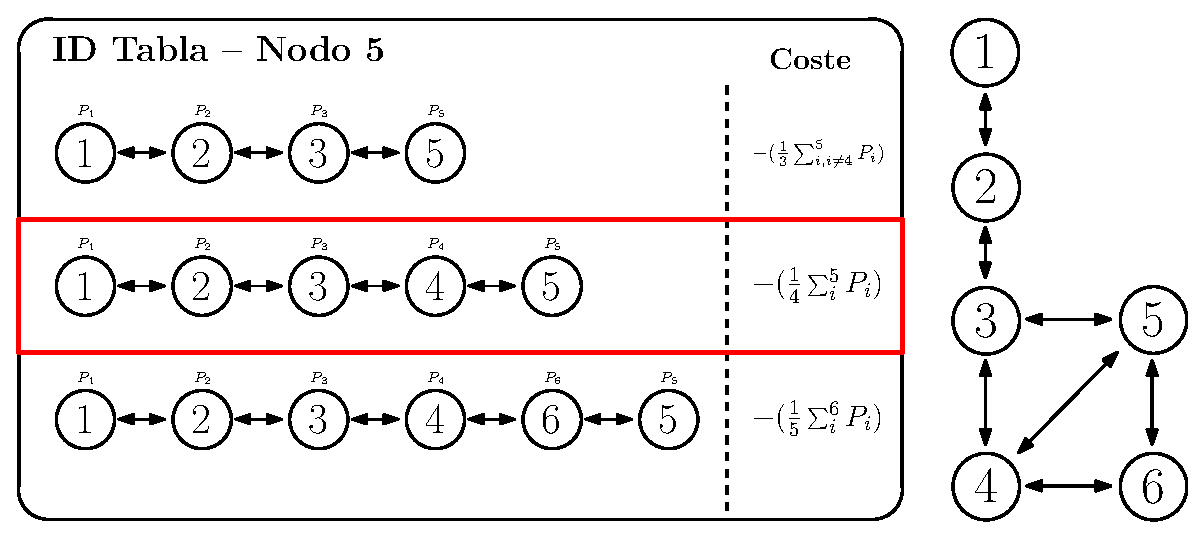
\includegraphics[width=0.9\textwidth]{fig/05_den2ne/den2ne_10.eps}
    \caption{Selección de ID basada en el criterio de balance de potencia ponderado.}
    \label{fig:den2ne_10}
\end{figure}


\subsection{Fase 3 - Balance global}
\label{subsec:fase3}

Una vez que las etiquetas se asignan a lo largo de toda la topología, se aplica un criterio determinado y cada nodo tiene un $ID_{activa}$, puede comenzar el procedimiento para equilibrar los recursos disponibles. El objetivo del algoritmo es alcanzar un estado de balance global trasladando recursos desde los nodos más alejados, hacia la raíz. Este movimiento se implementa de manera local, pero siguiendo un orden específico basado en el $ID_{activa}$ de cada nodo, lo que finalmente produce un equilibrio general de los recursos para todos los nodos de la topología. \\
\\
Para proceder, dado que el algoritmo es centralizado, es posible recopilar el $ID_{activa}$ de cada nodo y ordenarlos en función de su longitud. Cuanto más largo sea el $ID_{activa}$, más alejado estará el nodo, desde un punto de vista lógico, de la raíz\footnote{Es importante destacar el adverbio \textit{lógicamente} en este contexto, ya que el nodo podría estar físicamente más cerca, pero el $ID_{activa}$ seleccionado puede proporcionar una vista lógica diferente.}. Por lo tanto, el algoritmo comienza equilibrando la carga desde el $ID_{activa}$ más largo, que está asociado a un nodo específico de la red. En caso de que dos o más $ID_{activa}$ tengan la misma longitud, se seleccionará uno de ellos de manera aleatoria. Una vez que los nodos se ordenan en función de su $ID_{activa}$, el algoritmo visita cada nodo una sola vez para equilibrar el recurso con su nodo predecesor en la lista ordenada representada por el $ID_{activa}$. Considerando la terminología explicada en la sección~\ref{subsec:terminologiaDEN2NE}, las demandas se expresarán como un valor negativo y las ofertas como un valor positivo, siendo el objetivo dejar a cada nodo en un estado neutro (en este caso, sin demanda ni oferta implica un valor cero) y transferir la demanda u oferta restante al siguiente vecino de la lista. Este proceso se repite para cada nodo hasta llegar al último nodo de la lista (que corresponde al nodo con el $ID_{activa}$ más corto, es decir, el nodo raíz). En consecuencia, la raíz obtiene la oferta o demanda restante de toda la red, es decir, el balance global. Posteriormente, el nodo raíz, como nodo pasarela hacia el núcleo de la red, puede decidir por sí mismo qué hacer con dicha oferta o demanda sobrante. \\
\\
Para ejemplificar el procedimiento descrito, se presenta la Figura~\ref{fig:den2ne_11}, la cual, representa la topología de la red de ejemplo utilizada para explicar el algoritmo hasta el momento, en la cual el $ID_{activa}$ más largo es el asociado al nodo 5 (\texttt{1.2.3.4.6.5}). En consecuencia, la Figura~\ref{fig:den2ne_11} muestra la lista ordenada, donde el primer nodo a comprobar es el nodo 5, mientras que el último es el nodo 1. Para simplificar, en la figura solo se representan los $ID_{activa}$ de los tres primeros nodos que serán visitados (5, 6 y 4). En este escenario, el nodo 5 tiene una oferta de $3.1$, el nodo 6 tiene una demanda de $-1$, y el nodo 4 una oferta de $0.5$. Como el algoritmo comienza en el nodo 5, su estado se fijará en cero, y su oferta se transferirá al siguiente vecino en la lista, el nodo 6, que ahora actualizará sus recursos a $-1+3.1 \:= \:2.1$, tal como se muestra en la Figura~\ref{fig:den2ne_12}. Posteriormente, el siguiente nodo a procesar será el nodo 6 (\texttt{1.2.3.4.6}), que también se fijará en cero y su oferta o demanda se transferirá al siguiente nodo, de modo que el nodo 4 pase a tener $0.5+2.1 \: = \: 2.6$, como se ilustra en la Figura~\ref{fig:den2ne_13}. El algoritmo \gls{d2e} continúa procesando todos los nodos hasta llegar finalmente al nodo raíz, de manera que todos los nodos quedan equilibrados y el nodo raíz obtiene un valor global de oferta/demanda de la red.

% \begin{figure}[ht!]
%     \centering
%     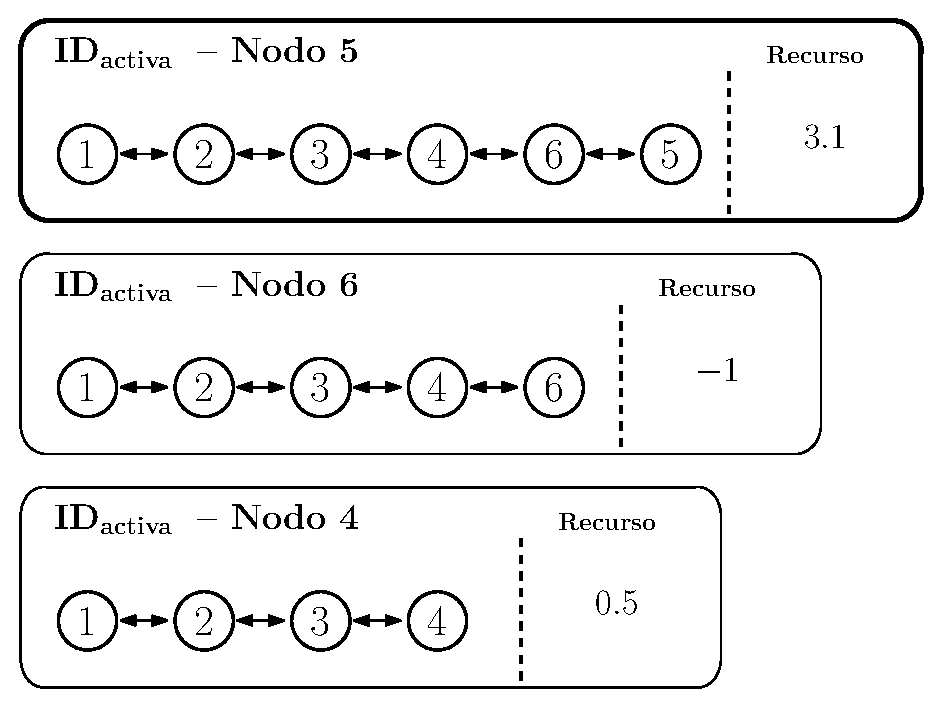
\includegraphics[width=0.55\textwidth]{fig/05_den2ne/den2ne_11.eps}
%     \caption{Ejemplo del procedimiento de balance global - Paso 1.}
%     \label{fig:den2ne_11}
% \end{figure}

% \begin{figure}[ht!]
%     \centering
%     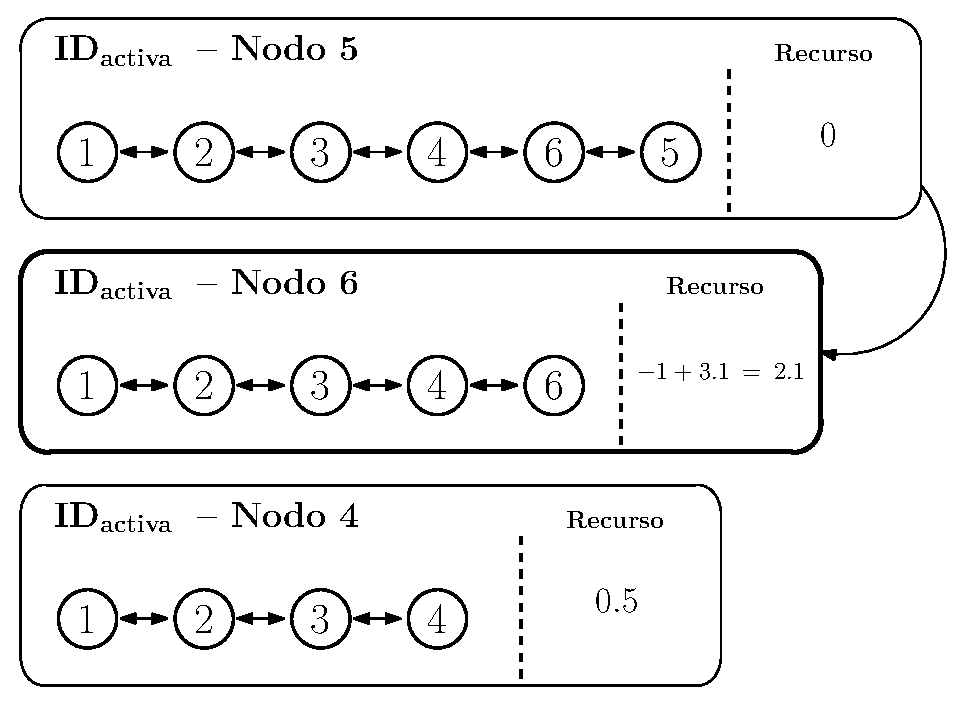
\includegraphics[width=0.55\textwidth]{fig/05_den2ne/den2ne_12.eps}
%     \caption{Ejemplo del procedimiento de balance global - Paso 2.}
%     \label{fig:den2ne_12}
% \end{figure}

% \begin{figure}[ht!]
%     \centering
%     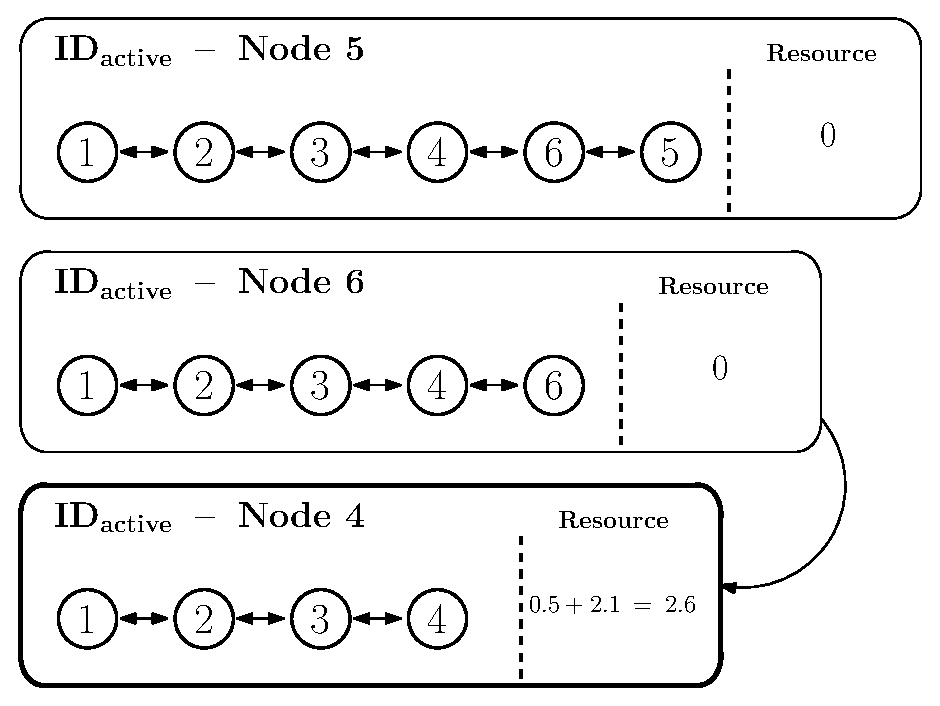
\includegraphics[width=0.55\textwidth]{fig/05_den2ne/den2ne_13.eps}
%     \caption{Ejemplo del procedimiento de balance global - Paso 3.}
%     \label{fig:den2ne_13}
% \end{figure}
\begin{figure}[H]
    \centering
    
    \begin{subfigure}{0.55\textwidth}
        \centering
        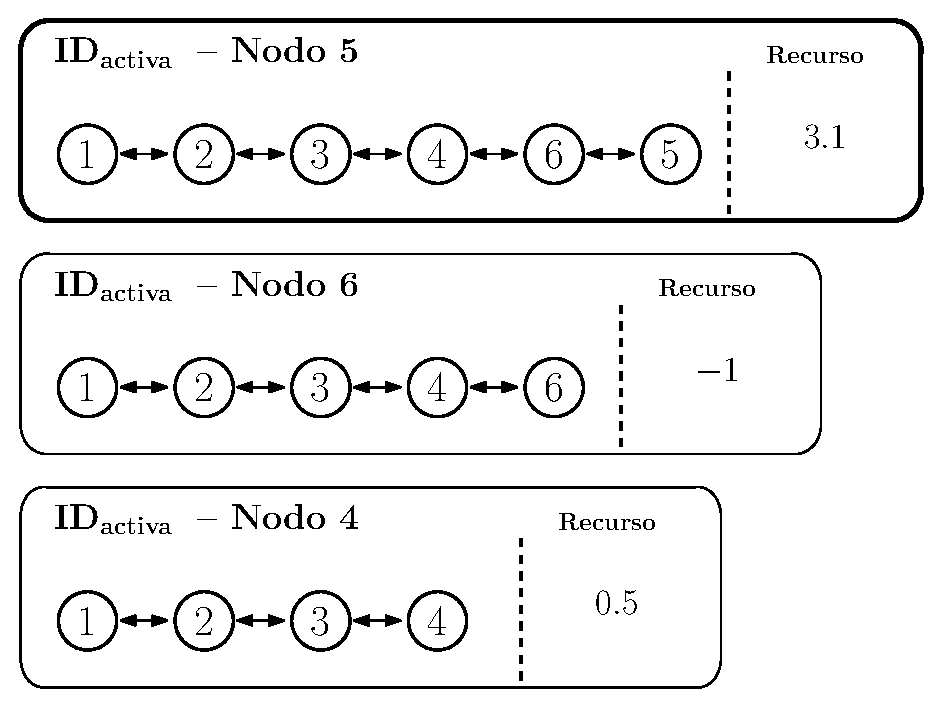
\includegraphics[width=\linewidth]{fig/05_den2ne/den2ne_11.eps}
        \caption{Paso 1.}
        \label{fig:den2ne_11}
    \end{subfigure}
    
    \vspace{0.3cm}
    
    \begin{subfigure}{0.55\textwidth}
        \centering
        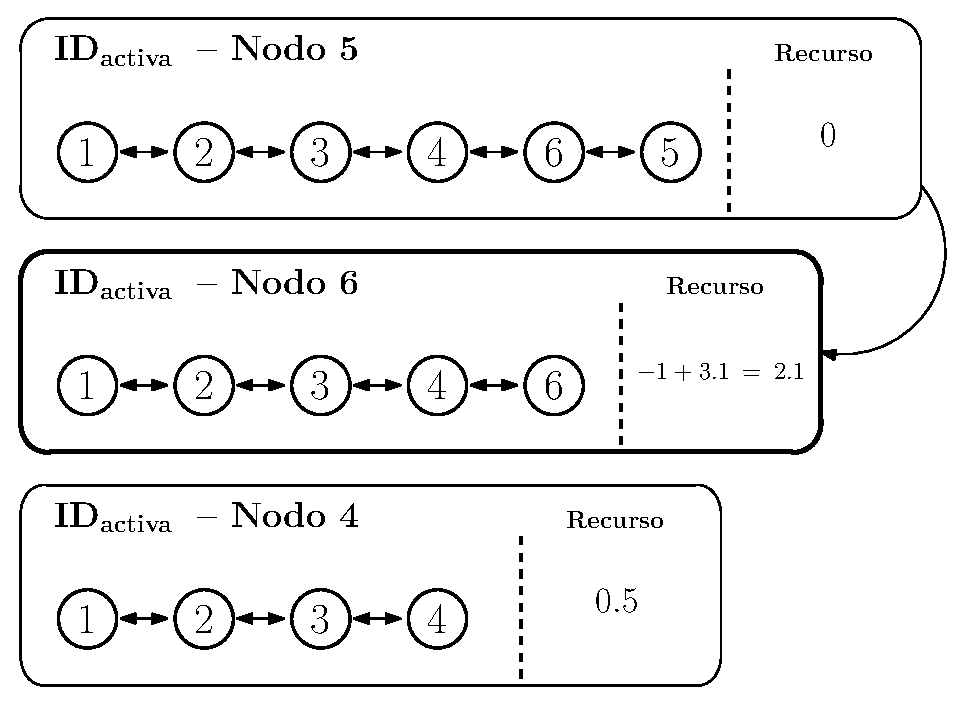
\includegraphics[width=\linewidth]{fig/05_den2ne/den2ne_12.eps}
        \caption{Paso 2.}
        \label{fig:den2ne_12}
    \end{subfigure}
    
    \vspace{0.3cm}
    
    \begin{subfigure}{0.55\textwidth}
        \centering
        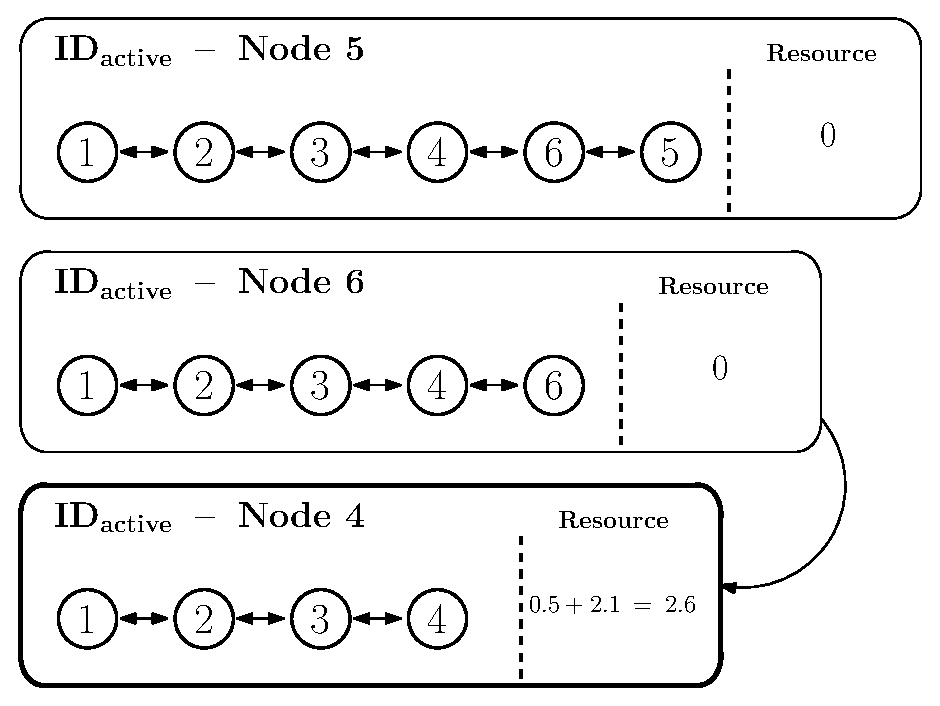
\includegraphics[width=\linewidth]{fig/05_den2ne/den2ne_13.eps}
        \caption{Paso 3.}
        \label{fig:den2ne_13}
    \end{subfigure}
    
    \caption{Ejemplo del procedimiento de balance global.}
    \label{fig:den2ne_balance}
\end{figure}


El procedimiento anterior se resume en el Algoritmo~\ref{alg:globalbalance}. Como se puede observar, las entradas del algoritmo son: (1) el grafo $G(\mathcal{N}, \mathcal{L})$, que es el conjunto de nodos de la topología ($\mathcal{N}$) y enlaces ($\mathcal{L}$), y (2) el $scenario\_type$, que puede ser uno de los siguientes cuatro (definidos únicamente como referencia para representar y, posteriormente, evaluar, distintos casos de uso): 


\begin{itemize}

    \item \textbf{Escenario ideal}: Representa un escenario en el que no existe pérdida de recursos durante la transmisión cuando el recurso ($r_{i}$) se envía de un nodo $i$ a otro $j$ ($i,j \in \mathcal{N} \: \:\forall \:\: i \neq j$) a través de un enlace sin pérdidas, es decir, $L_{ij} \: = 0$. En consecuencia, para cualquier transmisión de recursos $i \rightarrow j$, en la que el estado inicial es $\{i=r_{i},\: j=r_{j}\}$, los recursos resultantes tras la transmisión son $\{i' = 0,\: j' = r_{i}+r_{j}\}$.
    
    
    \item \textbf{Escenario con pérdidas}: Implica la existencia de pérdidas durante la transmisión de recursos, es decir, $L \: \neq \varnothing$. En consecuencia, para cualquier transmisión de recursos $i \rightarrow j$, en la que el estado inicial es $\{i=r_{i},\: j=r_{j}\}$, los recursos resultantes tras la transmisión son $\{i' = 0,\: j' = r_{i}+r_{j}-L_{ij}\}$. El modelo de pérdidas que se empleará está descrito en \cite{Schneider17}, utilizando las pérdidas de transmisión definidas en la Ecuación \ref{eq:criterionCost04_b}.
    
    
    \item \textbf{Escenario con capacidad de enlace restringida}: Hasta ahora, los enlaces no tenían ninguna limitación particular al transmitir un recurso, pero si el enlace está restringido a ciertos valores de transmisión, el recurso no se reenviará oportunamente y el excedente será descartado (al menos, de forma lógica para el algoritmo, incluso si el exceso de recurso permanece en su origen). Más específicamente, si la capacidad del enlace es $C_{ij}$, con $C \: \neq \varnothing$, y $r_{i} \geq C_{ij}$, entonces la transmisión de recursos asociada $i \rightarrow j$ con estado inicial $\{i=r_{i},\: j=r_{j}\}$ resultará en el estado final $\{i' = 0,\: j' = \: C_{ij}+r_{j}\}$. El modelo de las capacidades de los enlaces empleados está descrito en \cite{Schneider17}, donde se especifica que la capacidad máxima de cada enlace es $C_{max} \: = I_{max} \: \times \: V_{d}$.
    
    
    \item \textbf{Escenario con pérdidas y capacidad de enlace restringida}: Este último tipo combina los dos anteriores, es decir, $L \: \neq \varnothing$ y $C \: \neq \varnothing$. En consecuencia, para cualquier transmisión de recursos $i \rightarrow j$, en la que el estado inicial es $\{i=r_{i},\: j=r_{j}\}$, los recursos resultantes tras la transmisión son $\{i' = 0,\: j' = r_{i}+r_{j}-L_{ij}\}$ en caso de que $r_{i} \leq C_{ij}$, y $\{i' = 0,\: j' = C_{ij}+r_{j}-L_{ij}\}$ en caso de que $r_{i} \geq C_{ij}$.  
 
\end{itemize}

Con respecto a las salidas del Algoritmo~\ref{alg:globalbalance}, $total\_balance\_ideal$ proporciona el balance global de la topología (que corresponde a la carga final en la raíz, ya que esta permanece como el último nodo y conserva la diferencia de todas las transferencias de recursos; de ahí que $total\_balance \: = \: root.load$), mientras que $abs\_flux$ proporciona un valor absoluto de los intercambios de recursos a lo largo de la red (para cualquier intercambio se considera su valor absoluto, ya que el signo negativo o positivo solo indica la dirección, pero el movimiento de recursos ocurre en cualquier caso). \\
\\
Por lo tanto, $total\_balance$ expresa si la red presenta una demanda o un exceso global de recursos, mientras que $abs\_flux$ representa el cantidad de recursos distribuidos. 

\begin{algorithm}[ht!]
\caption{Proceso de balance global}\label{alg:globalbalance}
\SetKwInOut{Input}{input}
\SetKwInOut{Output}{output}
\Input{$\: G(\mathcal{N}, \mathcal{L}),\: scenario\_type$}
\Output{$\: total\_balance, \: abs\_flux$}
\vspace{0.2cm}
$\textup{init}\: global\_ids, abs\_flux$\;
$\textup{sort}\: global\_ids$\;
\vspace{0.1cm}
\While{$length(global\_ids) > 1$}{
\vspace{0.1cm}
    $origin \: = \: \mathcal{N}(global\_ids[0])$\;
    $destination \: = \: \textup{get next hop from} \:origin$\;
\vspace{0.1cm}  

  \eIf{$origin.load \: > 0$}{
    $\textup{setLinkDirection} \: \mathcal{L}(origin, \: destination) \: \textup{to down}$\;

  }{
    $\textup{setLinkDirection} \: \mathcal{L}(origin, \: destination) \: \textup{to up}$\;
  }


    \Switch{$scenario\_type$}{
        \Case{$ideal$}{ 
                $destination.load \: = destination.load \: + \: origin.load$\;
                $abs\_flux \: = abs\_flux  \: + \:\left |  origin.load \right |$\;
        }
        \Case{$lossy$}{
              $destination.load \: = destination.load \: + \: origin.load \: - \: \textup{losses}$\;
              $abs\_flux \: = abs\_flux  \: + \:\left |  origin.load  \: - \: \textup{losses}\right |$\;
        
        }
        \Case{$capacity$}{
            \eIf{$origin.load \geq capacity$}{
                $destination.load \: = destination.load \: + \: capacity$\;
                $abs\_flux \: = abs\_flux  \: + \:\left |  capacity \right |$\;
            }{
                $destination.load \: = destination.load \: + \: origin.load$\;
                $abs\_flux \: = abs\_flux  \: + \:\left |  origin.load \right |$\;
            }
        }
        \Other{
            \eIf{$origin.load \geq capacity$}{
                $destination.load \: = destination.load \: + \: capacity \: - \: \textup{losses}$\;
                $abs\_flux \: = abs\_flux  \: + \:\left |  capacity \: - \: \textup{losses} \right |$\;
            }{
                $destination.load \: = destination.load \: + \: origin.load \: - \: \textup{losses}$\;
                $abs\_flux \: = abs\_flux  \: + \:\left |  origin.load \: - \: \textup{losses} \right |$\;
            }
        }
    }

    %\vspace{0.1cm}
  $origin.load \: = \: \varnothing$\;
  $\textup{pop}\: global\_ids[0]$\;
  
}
%\vspace{0.1cm}
\Return{$root.load, abs\_flux$}
\end{algorithm}

Concretamente, $total\_balance$ podría ser igual o cercano a cero, lo cual significa que la red no tiene una demanda específica de recursos, pero $abs\_flux$ podría indicar un valor elevado, lo que evidencia que, para alcanzar un balance global, se requiere un alto número de intercambios. De hecho, $total\_balance$ simplemente ilustra la naturaleza del escenario (es decir, cantidad de ofertas frente a demandas), mientras que $abs\_flux$ constituye realmente un indicador de la eficacia del algoritmo, ya que cuanto menor sea su valor, menor será el coste para balancear óptimamente la carga de recursos en la topología.\\
\\
Como se puede observar, el Algoritmo~\ref{alg:globalbalance} es lineal (complejidad $\mathcal{O}(n)$), ya que los nodos de la red son visitados una sola vez considerando la etiqueta o identificador seleccionado en la segunda fase del algoritmo, lo cual queda representado por el único bucle ($while$) del mismo. Finalmente, cabe destacar que el algoritmo \gls{d2e} se ejecuta en base a una instantánea específica de la red. Si la red se actualiza debido a la movilidad de nodos, o a la modificación de ofertas y demandas, el algoritmo puede ejecutarse de nuevo, en cualquier momento, para redistribuir los nuevos recursos.

\section{Entorno de evaluación}
\label{sec:den2ne_setup}
La implementación y configuración de la evaluación están basadas en Python 3.8\footnote{\url{https://peps.python.org/pep-0569/}}. Más específicamente, la evaluación se divide en dos etapas:

\begin{enumerate}
    \item Un generador de topologías aleatorias para probar exhaustivamente \gls{d2e}, que aprovecha el entorno \gls{brite}~\cite{brite}, como se muestra en la Figura~\ref{fig:den2ne_14} (el cual traduce los archivos \texttt{*.brite} en archivos \texttt{*.csv} para los nodos y enlaces de la topología, utilizados como entrada en nuestro algoritmo).
   
    \item La ejecución del algoritmo, desarrollado como un script centralizado, que importa todas las topologías generadas, una por una, utilizando semillas y diferentes parámetros de \gls{d2e} para su comparación. 
\end{enumerate}

\begin{figure}[ht!]
    \centering
    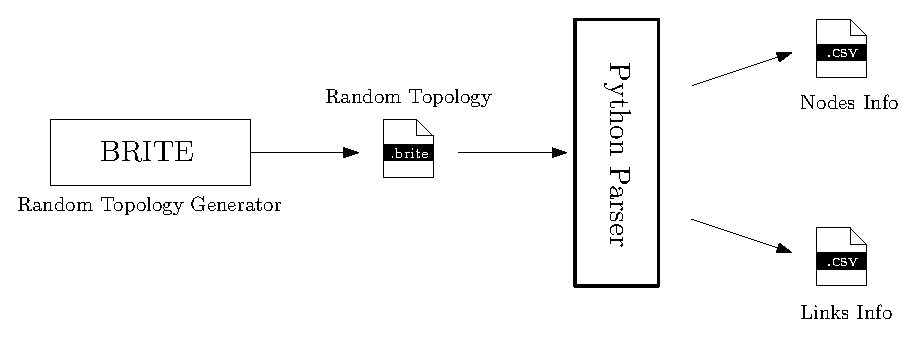
\includegraphics[width=0.7\textwidth]{fig/05_den2ne/den2ne_14.eps}
    \caption{Generador de topologías para DEN2NE basado en BRITE.}
    \label{fig:den2ne_14}
\end{figure}

Nuestro objetivo es proporcionar un análisis exhaustivo del algoritmo \gls{d2e}, abarcando la mayor cantidad posible de tipos de escenarios. De hecho, los grafos proporcionados por \gls{brite} se basan en topologías aleatorias Waxman~\cite{waxman1988routing} y Barabási-Albert~\cite{barabasi1999emergence}, las cuales se emplean para modelar una amplia gama de sistemas de interconexión, desde redes de computación, a redes de comunicaciones, y hasta redes sociales. La red aleatoria Waxman se fundamenta en un modelo probabilístico para la generación aleatoria de una red, mientras que la red Barabási-Albert se enmarca dentro de la categoría de redes \textit{scale-free} (también conocidas como redes \textit{hub-and-spoke}), en las cuales ciertos nodos presentan un número de conexiones significativamente mayor que el resto. Una vista simplificada de ambos modelos se muestra en la Figura~\ref{fig:den2ne_15}.

\begin{figure}[ht!]
    \centering
    \begin{subfigure}[t]{0.45\textwidth}
        \centering
        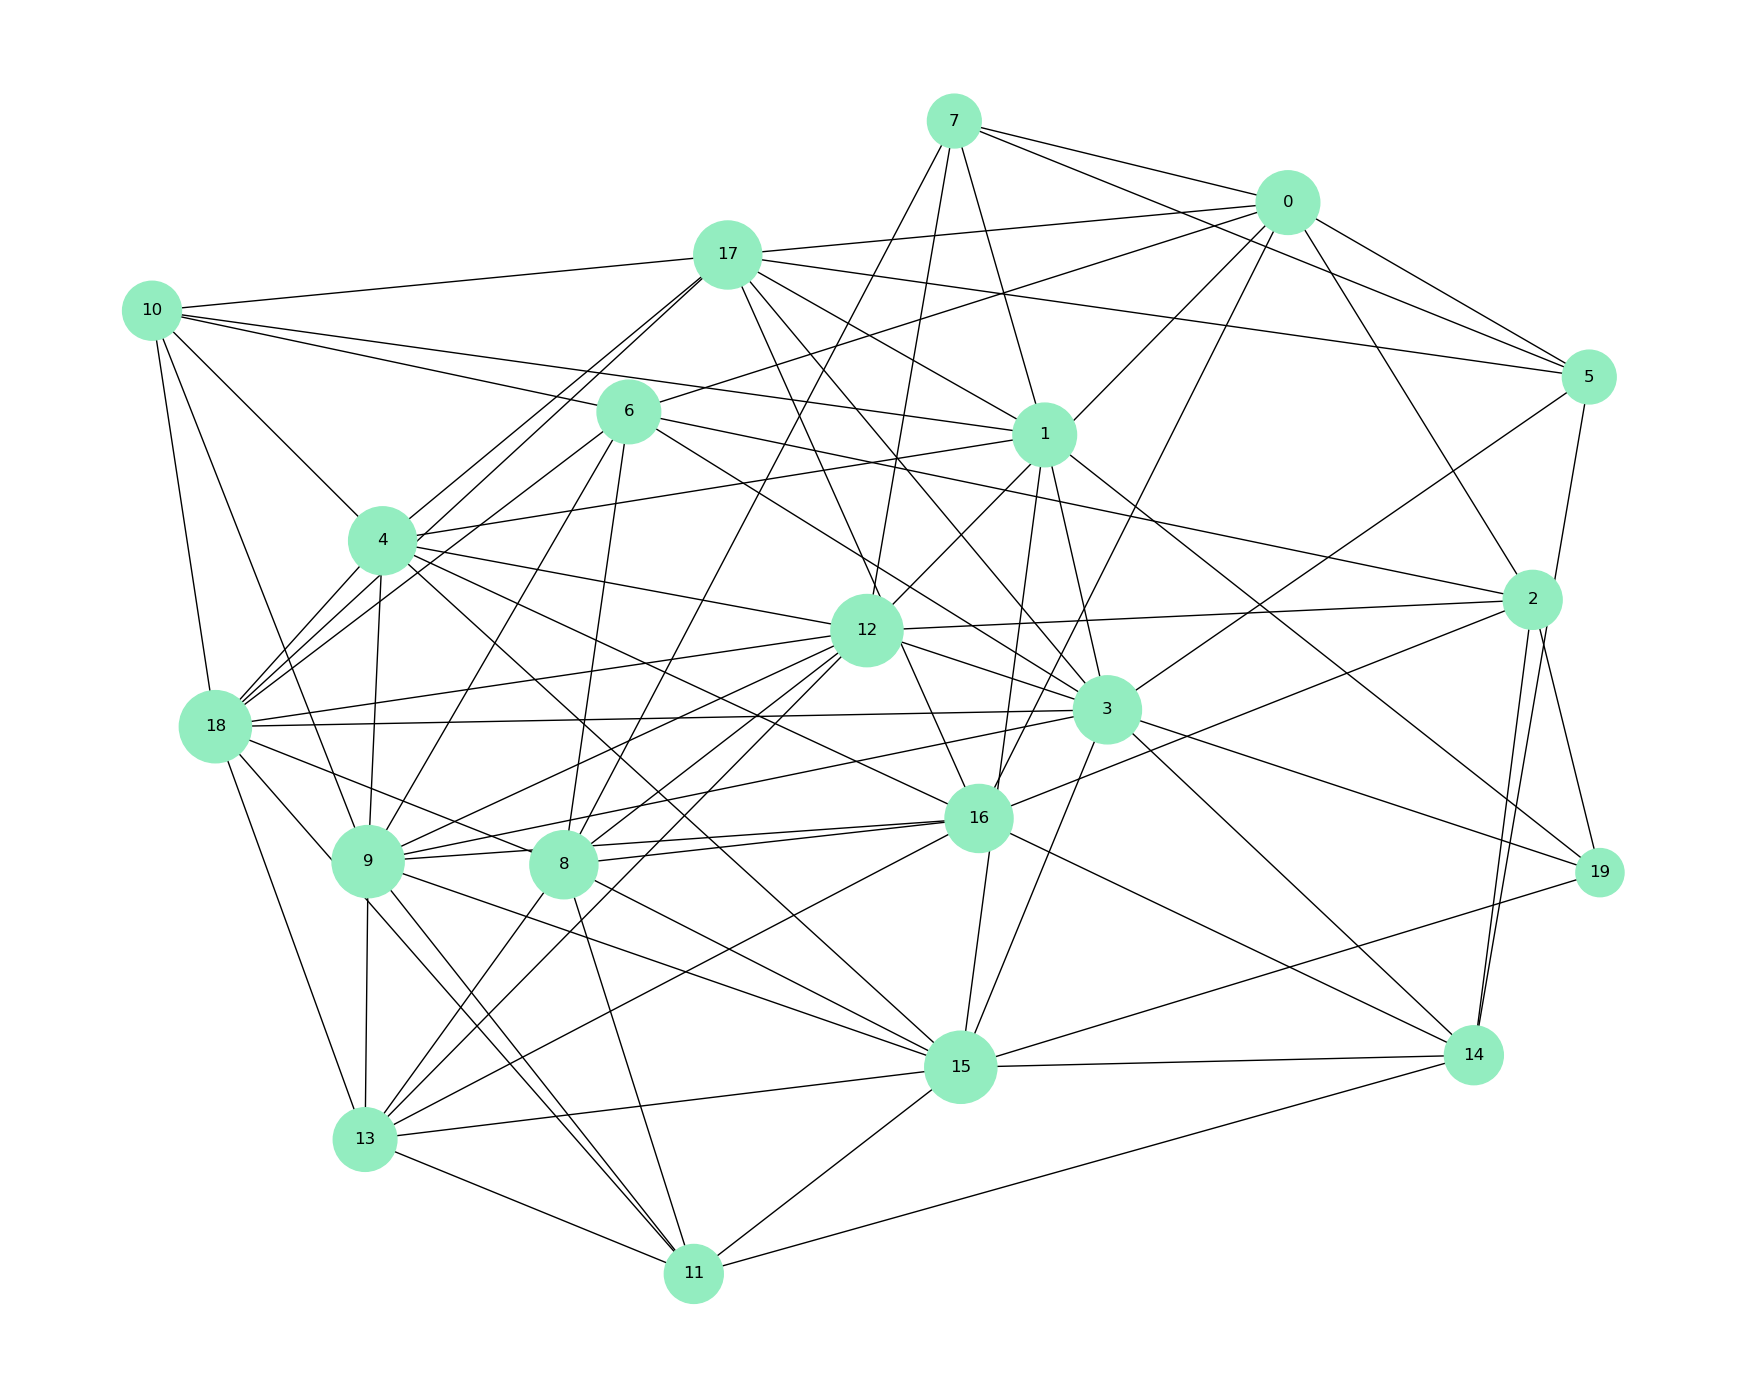
\includegraphics[width=\linewidth]{fig/05_den2ne/den2ne_15a.png}
        \caption{Topología Waxman}
        \label{fig:waxman}
    \end{subfigure}
    \hfill
    \begin{subfigure}[t]{0.45\textwidth}
        \centering
        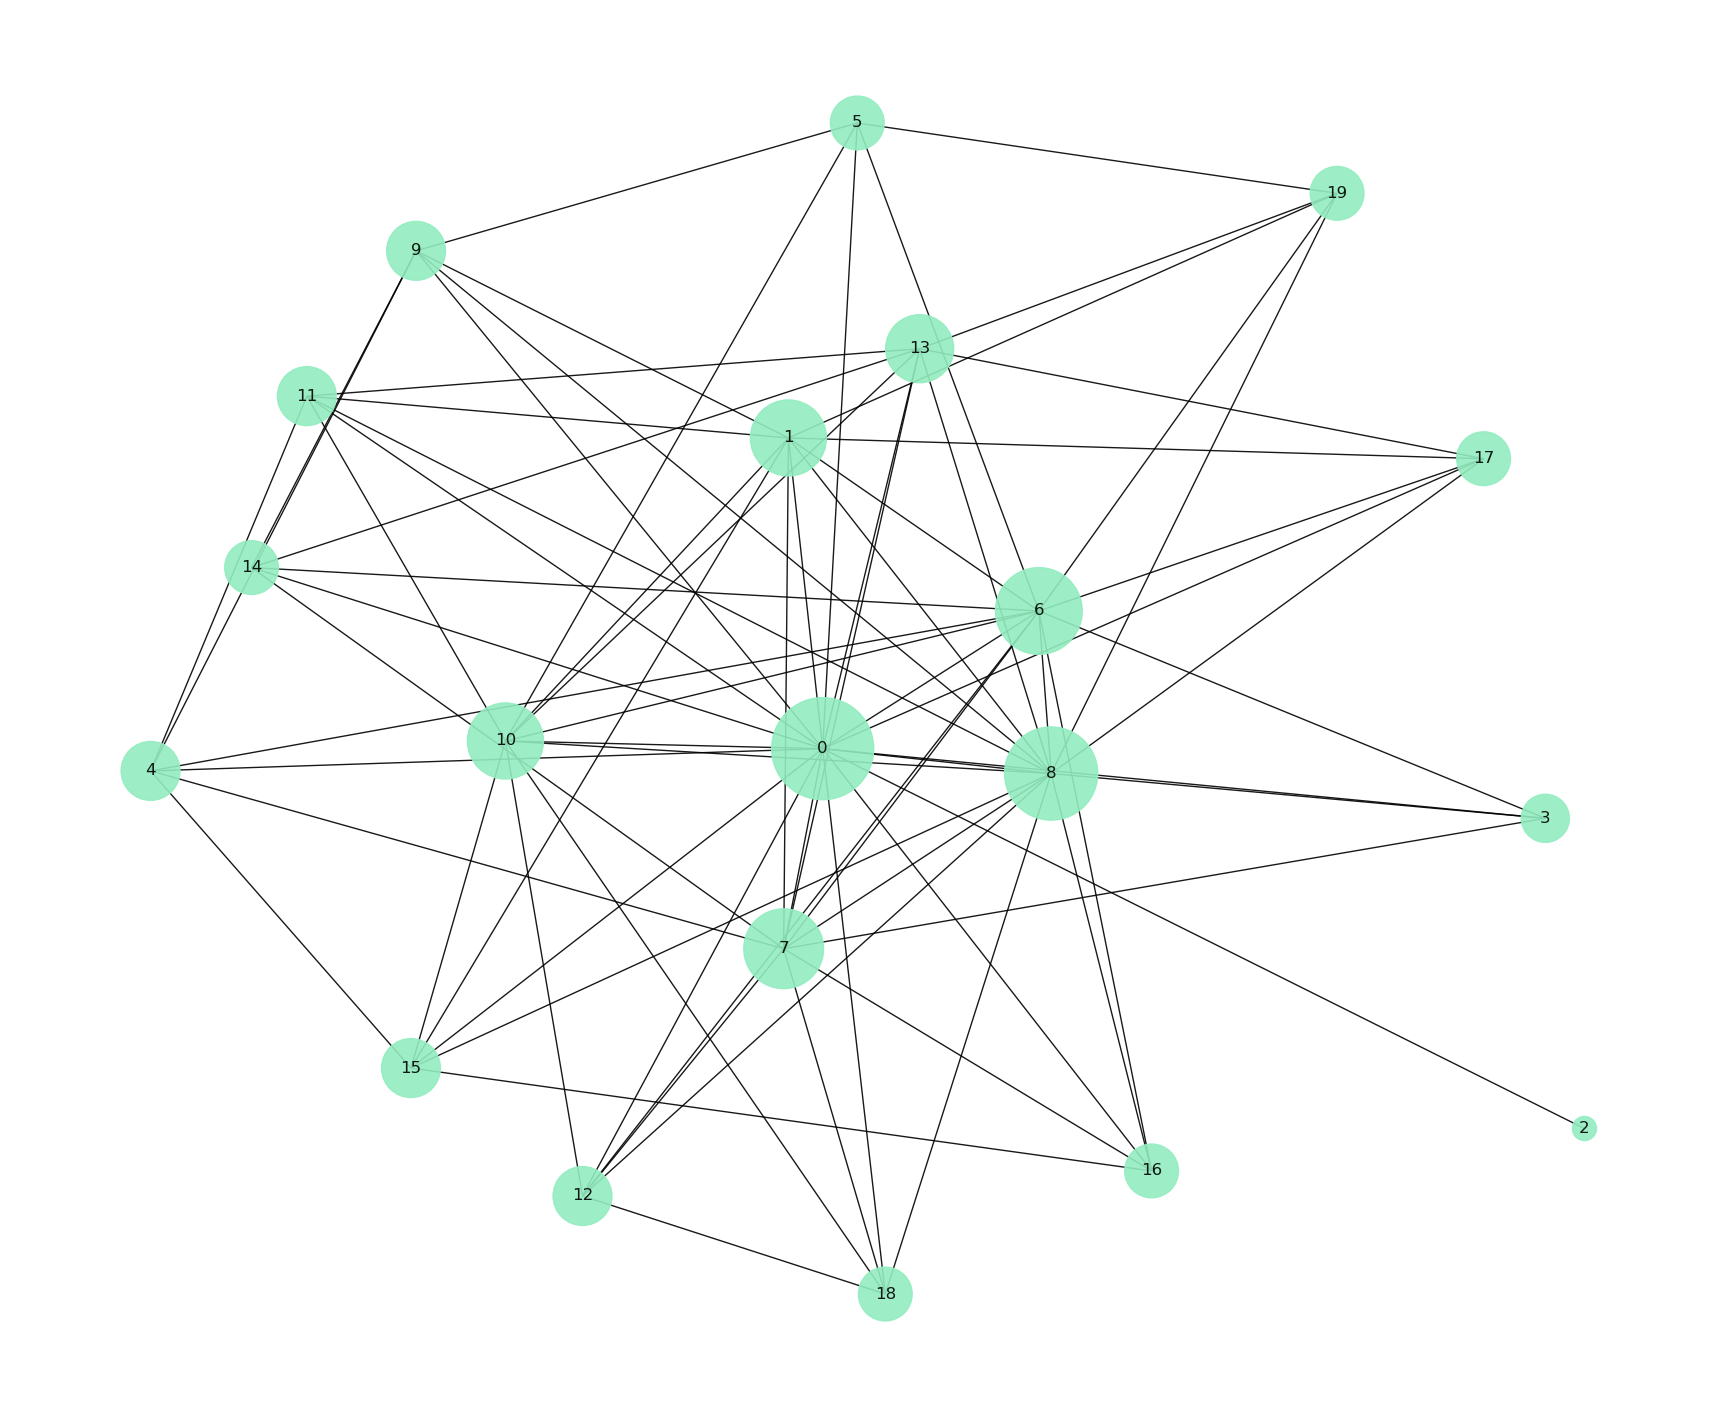
\includegraphics[width=\linewidth]{fig/05_den2ne/den2ne_15b.png}
        \caption{Topología Barabási-Albert}
        \label{fig:barabasi}
    \end{subfigure}
    \caption{Topologías aleatorias empleadas en el estudio de DEN2NE.}
    \label{fig:den2ne_15}
\end{figure}

En lo que respecta a los parámetros de generación de topologías, estos se resumen en la Tabla~\ref{tab:topologyParams}, la cual incluye: tipo de topología (uno de los dos tipos mencionados anteriormente), número de nodos (de 10 a 200 nodos en intervalos de 10 nodos), grado de conectividad (número promedio de enlaces por nodo, de 4 a 6, en intervalos de 2 enlaces) y una semilla de topología aleatoria (para obtener 10 topologías aleatorias de cada tipo). De acuerdo con estos parámetros, el número total de topologías evaluadas fue de 1200, tal y como se indica en la Ecuación~\ref{eq:numtopos}.


\begin{table}[ht!]
\centering
\begin{tabular}{|l|c|}
\hline
\multicolumn{1}{|c|}{\textbf{Atributos}} & \textbf{Valores} \\ \hline
Tipo de topología & {[}"\texttt{waxman}", "\texttt{barabasi-albert}"{]} \\ \hline
Número de nodos & {[}\texttt{10:10:200}{]} \\ \hline
Grado de conectividad & {[}\texttt{4:2:6}{]} \\ \hline
Semillas de las topologías aleatorias & {[}\texttt{1:1:10}{]} \\ \hline
\end{tabular}
\vspace{0.2cm}
\caption{Parámetros de generación de las topologías aleatorias.}
\label{tab:topologyParams}
\end{table}

\begin{equation}\label{eq:numtopos}
\begin{split}    
    \left \langle N_{topos} \right \rangle  \: & = { \: N_{tipo} \: \times \: N_{nodos} \: \times \:  N_{grado} \: \times \: N_{semilla}} \\
    & = 2 \times 20 \times 3 \times 10 \: = \: 1200 \: \: topos
\end{split}
\end{equation}
\vspace{0.2cm}

La evaluación realizada tiene como objetivo comparar el comportamiento de los 6 criterios descritos en la Sección~\ref{subsec:fase2} en cuatro tipos de escenarios de red (ideal, con pérdidas, con capacidad de enlace restringida y con capacidad de enlace restringida y pérdidas). Adicionalmente, el banco de pruebas debía asignar una oferta o demanda inicial de recursos a cada nodo de la topología. Esta asignación de recursos fue agnóstica (no se asocia ninguna unidad o métrica en particular) y podía estar limitada a un valor total determinado (fijado en 250, asumiendo al menos 1 unidad de recurso por nodo en promedio en las topologías más grandes) o no estarlo (sin un valor máximo establecido). La limitación en la asignación de recursos se definió con el fin de depurar la implementación y el comportamiento del algoritmo en los escenarios más complejos. En cualquier caso, tanto en la versión limitada como en la no limitada, la carga asignada a cada nodo siguió una distribución uniforme, como se ilustra en la Figura~\ref{fig:den2ne_16}.

\begin{figure}[ht!]
    \centering
    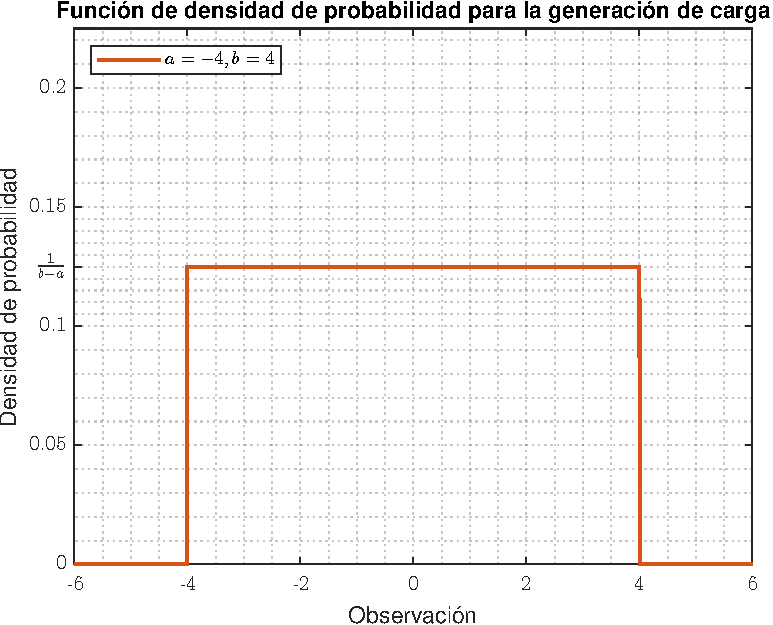
\includegraphics[width=0.7\textwidth]{fig/05_den2ne/den2ne_16.pdf}
    \caption{Función de densidad de probabilidad para la generación de cargas aleatorias en cada topología.}
    \label{fig:den2ne_16}
\end{figure}

Finalmente, para validar nuestros resultados, cada escenario se repitió 10 veces utilizando diferentes semillas para la generación aleatoria de recursos. Estas semillas solo modificaban la ubicación de la raíz y la asignación de recursos, mientras que el resto del escenario se mantenía igual, con el fin de demostrar exhaustivamente la validez de los resultados obtenidos. Todos estos parámetros se resumen en la Tabla~\ref{tab:testparams}. Por lo tanto, el número total de simulaciones de nuestro estudio es de 576000, tal y como se indica en la Ecuación~\ref{eq:numsim}.


\begin{equation}\label{eq:numsim}
\begin{aligned}
    \left \langle N_{simulaciones} \right \rangle  \: & = \: { N_{topos} \: \times \: N_{criterios} \: \times \:  N_{escenarios} \: \times \: N_{LR} \: \times \: N_{semilla}} \\ \: & = 1200 \times 6 \times 4 \times 2 \times 10 \\
    \: & = \: 576000 \: \: simulaciones
\end{aligned}    
\end{equation}
\vspace{0.2cm}

\begin{table}[ht!]
\centering
\begin{tabular}{|l|c|}
\hline
\multicolumn{1}{|c|}{\textbf{Atributo}} & \textbf{Valores} \\ \hline
Criterios & {[}\texttt{1:1:6}{]} \\ \hline
Tipo de escenario & {[}\texttt{1:1:4}{]} \\ \hline
Limitación de recursos & {[}\texttt{0,1}{]} \\ \hline
Semilla de ejecución aleatoria & {[}\texttt{1:1:10}{]} \\ \hline
\end{tabular}
\vspace{0.2cm}
\caption{Parámetros para la ejecución de pruebas.}
\label{tab:testparams}
\end{table}

\section{Resultados y evaluación del algoritmo}

Considerando la implementación y el entorno de evaluación presentados en la Sección~\ref{sec:den2ne_setup}, en esta sección se exponen los resultados obtenidos a partir de las simulaciones descritas. Para evaluar el comportamiento de \gls{d2e}, se midieron tres métricas diferentes: la primera en relación con el balance de recursos (que corresponde a una de las salidas del algoritmo \gls{d2e}, tal y como se describió previamente en el Algoritmo~\ref{alg:globalbalance}), y las otras dos en relación con el tiempo de ejecución, tanto para la asignación de etiquetas como para el balance de recursos, ya que nuestro objetivo era evaluar qué tan eficiente es \gls{d2e} equilibrando la carga y qué tan rápido realiza dicha tarea. Por este motivo, las siguientes tres secciones examinan estos parámetros en detalle, considerando el tamaño, tipo y conectividad de la red, el tipo de escenario y los seis criterios definidos en la Sección~\ref{subsec:fase2}. Todas las métricas se han obtenido mediante múltiples repeticiones, tal y como se indicó en la Sección~\ref{sec:den2ne_setup}, e incluyen su respectiva desviación estándar, aunque esta resulta despreciable en la mayoría de los gráficos. Aunque se han llevado a cabo simulaciones en todos los casos posibles, con el fin de facilitar la interpretación de los resultados, la representación gráfica se ha restringido únicamente a los más representativos.\\
\\
Es importante destacar que la validez de los resultados presentados en esta sección está limitada a la implementación realizada en la Sección~\ref{sec:den2ne_setup}. En la práctica, si el escenario incluyera un controlador centralizado de software, podríamos obtener resultados muy similares. No obstante, por ejemplo, deberían añadirse los tiempos de comunicación entre el controlador y los demás nodos de la red, los cuales dependerían de condiciones completamente ajenas al algoritmo en sí.

\subsection{Flujo de balance de recursos} 

El flujo de balance de recursos representa la cantidad de recursos transferidos entre todos los nodos de la topología. Esta métrica se ha calculado sumando todos los intercambios de recursos entre pares de nodos en valor absoluto, y fue presentada previamente en el Algoritmo~\ref{alg:globalbalance} como la variable \textit{abs\_flux}. Esta métrica indica el coste de equilibrar los recursos: cuanto mayor sea su valor, más costoso resulta dicho balance.\\


\begin{figure}[H]
    \centering
    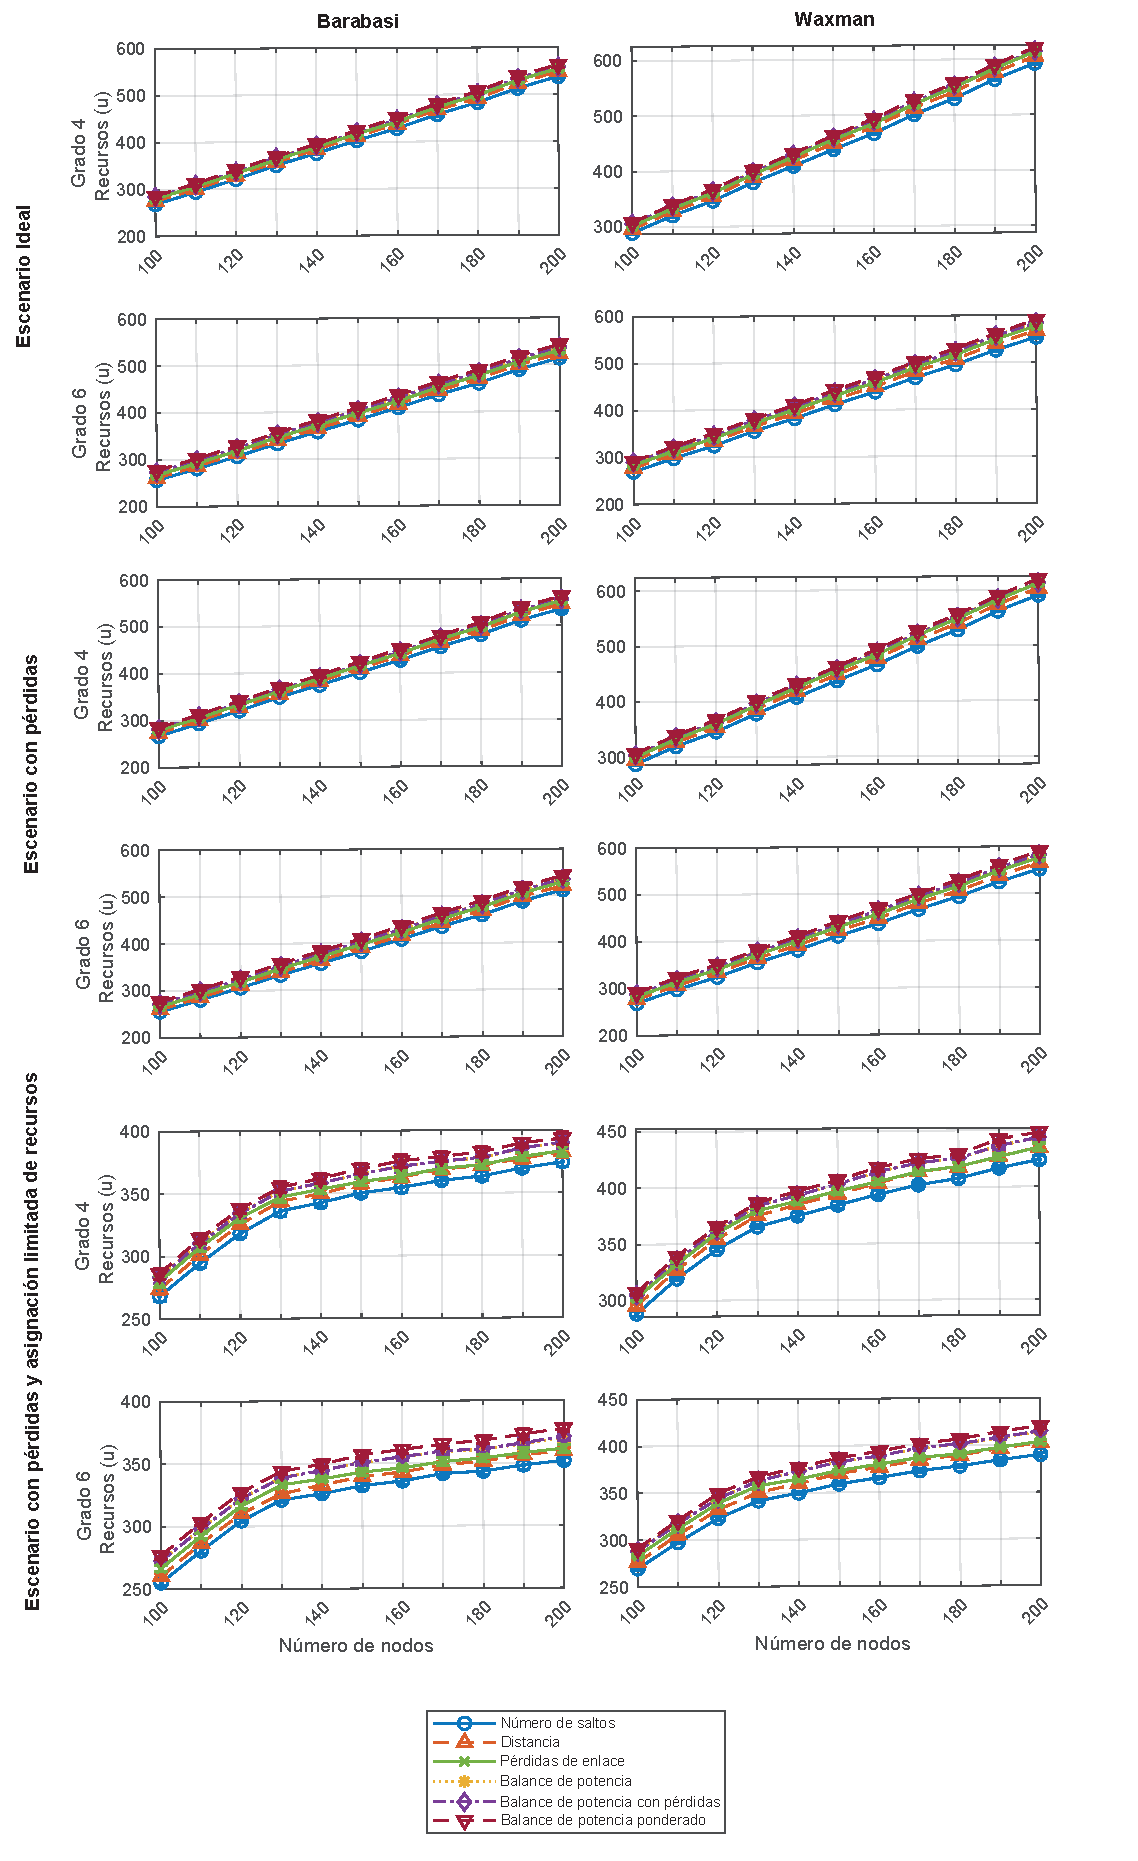
\includegraphics[width=0.85\textwidth,angle=0.9]{fig/05_den2ne/den2ne_17.pdf}
    \caption{Flujo de balance de recursos (\textit{abs\_flux}) - Tres escenarios y dos grados de red.}
    \label{fig:f1}
\end{figure}

La Figura~\ref{fig:f1} ilustra el flujo de balance de recursos para redes con grados de conectividad de 4 a 6, basadas en topologías de Barabási y Waxman, con tamaños comprendidos entre 100 y 200 nodos, y evaluadas con los seis criterios definidos en tres tipos de escenarios: ideal, con pérdidas y con pérdidas bajo limitación de asignación de recursos, respectivamente. Como puede observarse, el flujo crece de manera lineal con el tamaño de la topología, lo que indica que el algoritmo presenta un comportamiento escalable ($\mathcal{O}(n)$), sin estar fuertemente condicionado por el número de nodos involucrados. Únicamente en el último escenario, representado por los cuatro gráficos situados en la parte inferior de la Figura~\ref{fig:f1}, se aprecia un crecimiento de tipo logarítmico, aunque este efecto se debe a la limitación impuesta en la asignación de recursos.\\
\\
Adicionalmente, considerando los seis criterios, parece que el Criterio 1 (número de saltos) ofrece mejores resultados (menor flujo) que el resto, especialmente en topologías Waxman y cuando la conectividad de los nodos aumenta; mientras que el Criterio 6 (balance de potencia ponderado) se presenta como la peor opción, independientemente del escenario (incluso en los casos con pérdidas o con limitaciones de recursos). La discrepancia entre estos criterios puede explicarse por el hecho de que aquellos orientados a minimizar la distancia o el número de saltos hacia el nodo raíz favorecen trayectorias más cortas, mientras que los que consideran la cantidad de recursos a lo largo del camino hacia la raíz tienden a seleccionar trayectorias más largas. Por esta razón, en el Criterio 1 y el Criterio 2 (número de saltos y distancia, respectivamente), el flujo medio de recursos es menor en comparación con el Criterio 3 y el Criterio 6 (balance de potencia y balance de potencia ponderado, respectivamente), donde las trayectorias tienden a ser más largas en promedio, resultando en un mayor flujo de recursos.\\
\\
De la misma forma, la Figura~\ref{fig:f2} ilustra el balance total de recursos para redes con grados de conectividad de 4 a 6, basadas en topologías de Barabási y Waxman, con tamaños comprendidos entre 100 y 200 nodos, y evaluadas con los seis criterios definidos en tres tipos de escenarios: ideal, con pérdidas y con pérdidas bajo limitación de asignación de recursos, respectivamente. Como puede observarse, el balance total de recursos tiende a $0$ en todos los casos, lo cual resulta coherente si se considera que la asignación de recursos sigue la función previamente mostrada en la Figura~\ref{fig:den2ne_16}, cuyo valor medio es $0$. Además, en el escenario ideal todos los criterios producen el mismo resultado, y únicamente en los escenarios con pérdidas se observa cierta variabilidad, debido a que los caminos hacia la raíz (y, por tanto, las pérdidas) difieren. Esto indica que el algoritmo es capaz de compensar todos los recursos en la red, es decir, que todos los nodos tiendan hacia el valor cero (un uso óptimo), poniendo de manifiesto una distribución eficiente, dado que en pocos casos el nodo que actúa como pasarela (root) tendrá que demandar o verter excedentes en niveles superiores de la red.


\begin{figure}[H]
    \centering
    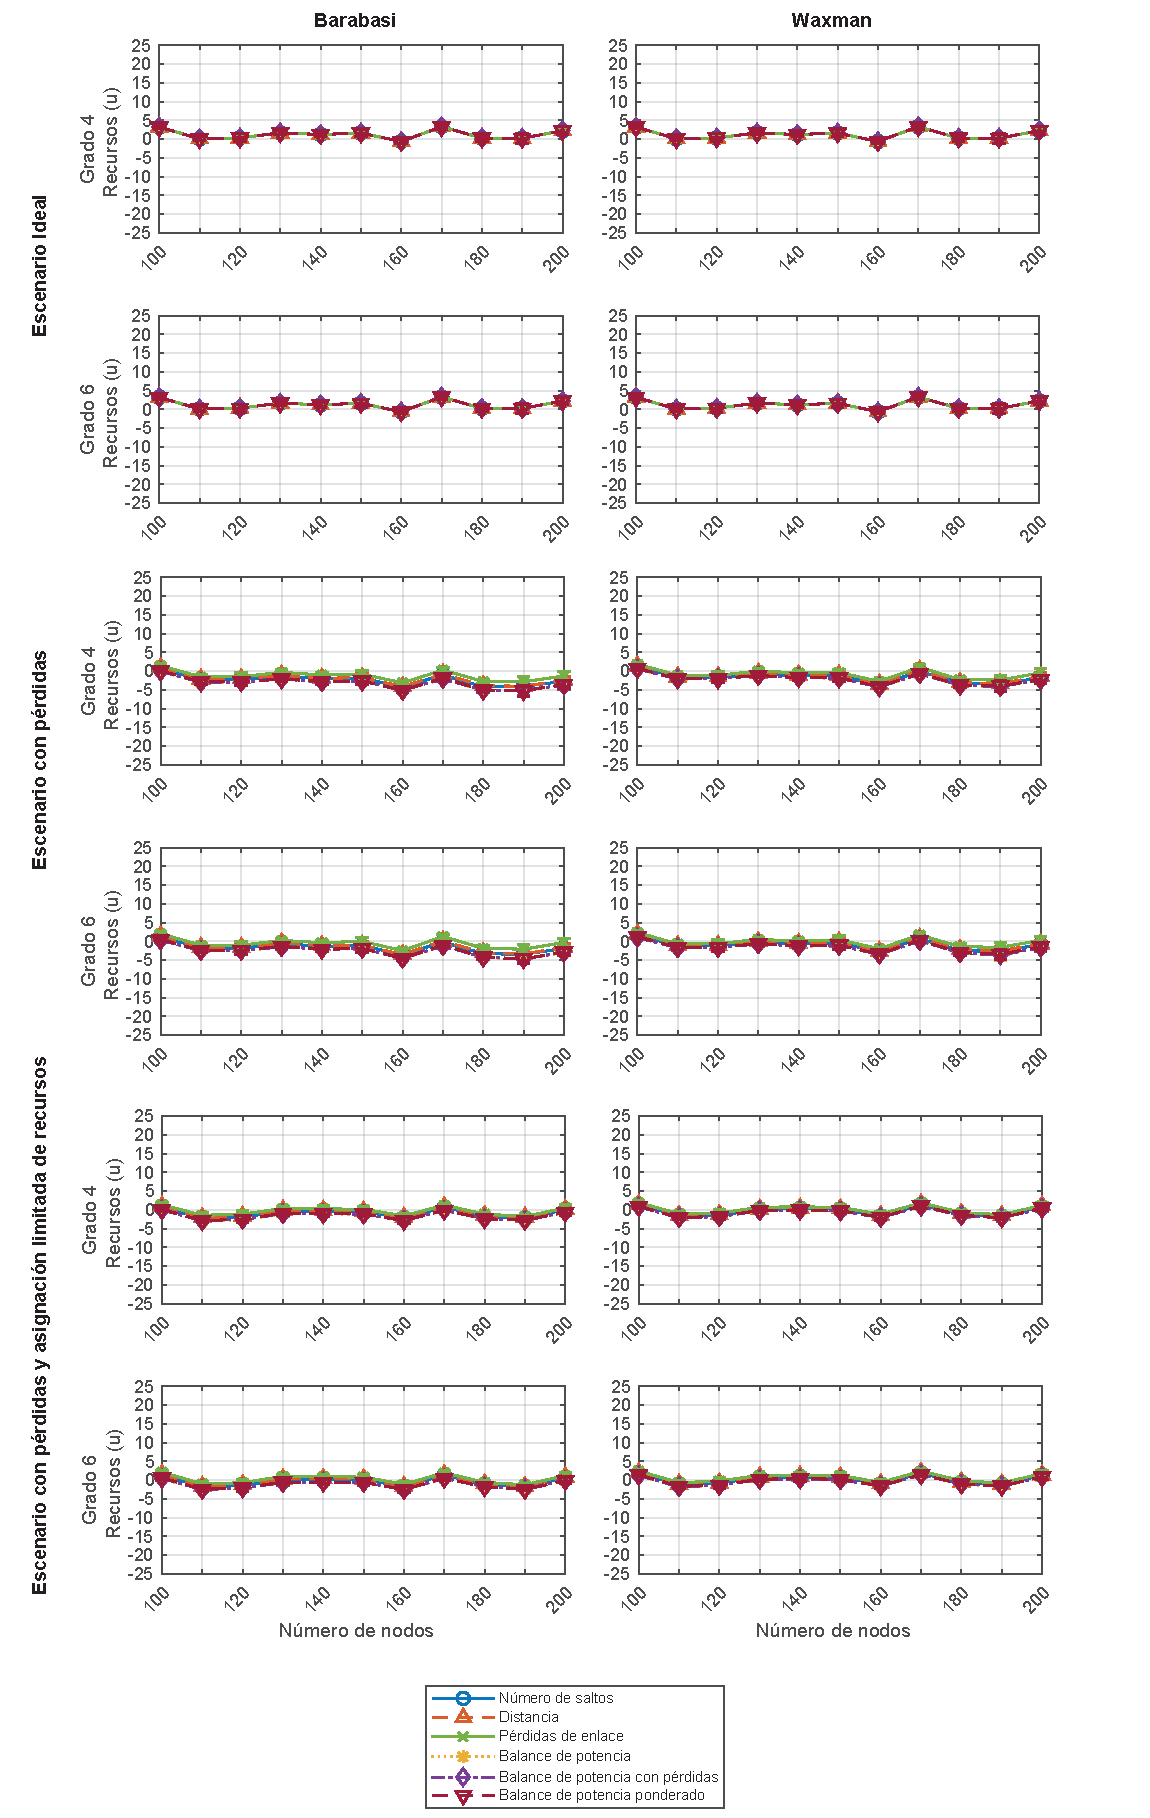
\includegraphics[width=0.85\textwidth,angle=0.9]{fig/05_den2ne/den2ne_18.pdf}
    \caption{Balance total de recursos (\textit{total\_balance}) - Tres escenarios y dos grados de red.}
    \label{fig:f2}
\end{figure}

\subsection{Tiempo de convergencia de la asignación de etiquetas} 

El tiempo de convergencia en la asignación de etiquetas representa el tiempo requerido por el algoritmo para asignar todas las etiquetas jerárquicas desde la raíz hasta el resto de los nodos de la topología. La Figura~\ref{fig:f4} muestra el tiempo de convergencia de la asignación de etiquetas para redes con grados de conectividad de 4 a 6, basadas en topologías de Barabási y Waxman, con tamaños comprendidos entre 100 y 200 nodos, y evaluadas con los seis criterios definidos en tres tipos de escenarios: ideal, con pérdidas y con pérdidas bajo limitación en la asignación de recursos, respectivamente.\\
\\
Como puede observarse, este tiempo de convergencia crece linealmente con el tamaño de la topología, sin verse afectado exponencialmente por el grado de conectividad u otros parámetros. Este hecho refleja una buena escalabilidad potencial del algoritmo, ya que, incluso en los peores casos, el tiempo de convergencia no supera los 15 ms. Además, los seis criterios presentan comportamientos muy similares, sin diferencias significativas. Esto se debe a que el tiempo de convergencia en la asignación de etiquetas depende estrictamente de la primera fase del algoritmo, la cual es independiente del criterio aplicado posteriormente. En caso de existir pequeñas variaciones, estas podrían atribuirse a la naturaleza aleatoria de las pruebas realizadas.


\subsection{Tiempo de convergencia del balance de recursos} 

El tiempo de convergencia en el balanceo de recursos representa el tiempo requerido por el algoritmo para realizar todos los intercambios de recursos hasta que la topología quede balanceada con respecto a la raíz. De igual forma, la Figura~\ref{fig:f3} muestra el tiempo de convergencia del balanceo de recursos para redes con grados de conectividad de 4 a 6, basadas en topologías de Barabási y Waxman, con tamaños comprendidos entre 100 y 200 nodos, y evaluadas con los seis criterios definidos en tres tipos de escenarios: ideal, con pérdidas y con pérdidas bajo limitación en la asignación de recursos, respectivamente. Como puede observarse, y de manera similar al tiempo de convergencia de la asignación de etiquetas, el tiempo de convergencia del balanceo de recursos crece linealmente con el tamaño de la topología, sin verse afectado de forma exponencial por el grado de conectividad u otros parámetros. Este hecho refleja una buena escalabilidad potencial del algoritmo, ya que, incluso en los peores casos, el tiempo de convergencia no supera 1 ms. En consecuencia, el tiempo total de ejecución del algoritmo \gls{d2e} fue inferior a 20 ms en todos los escenarios evaluados.\\
\\
Además, al igual que en la métrica de tiempo anterior, los seis criterios presentan comportamientos muy similares. En este caso, el tiempo de convergencia del balanceo de recursos sí depende de los criterios (a diferencia de la asignación de etiquetas), aunque la propia definición del algoritmo tiene un mayor impacto en este tiempo que el criterio seleccionado. Este aspecto resulta particularmente relevante, ya que los criterios se definen para favorecer una mejor asignación de recursos en distintos escenarios. Por lo tanto, estos resultados demuestran que nuestro algoritmo puede ajustarse y adaptarse a casos de uso específicos sin experimentar variaciones significativas en el tiempo de ejecución. 

\begin{figure}[H]
    \centering
    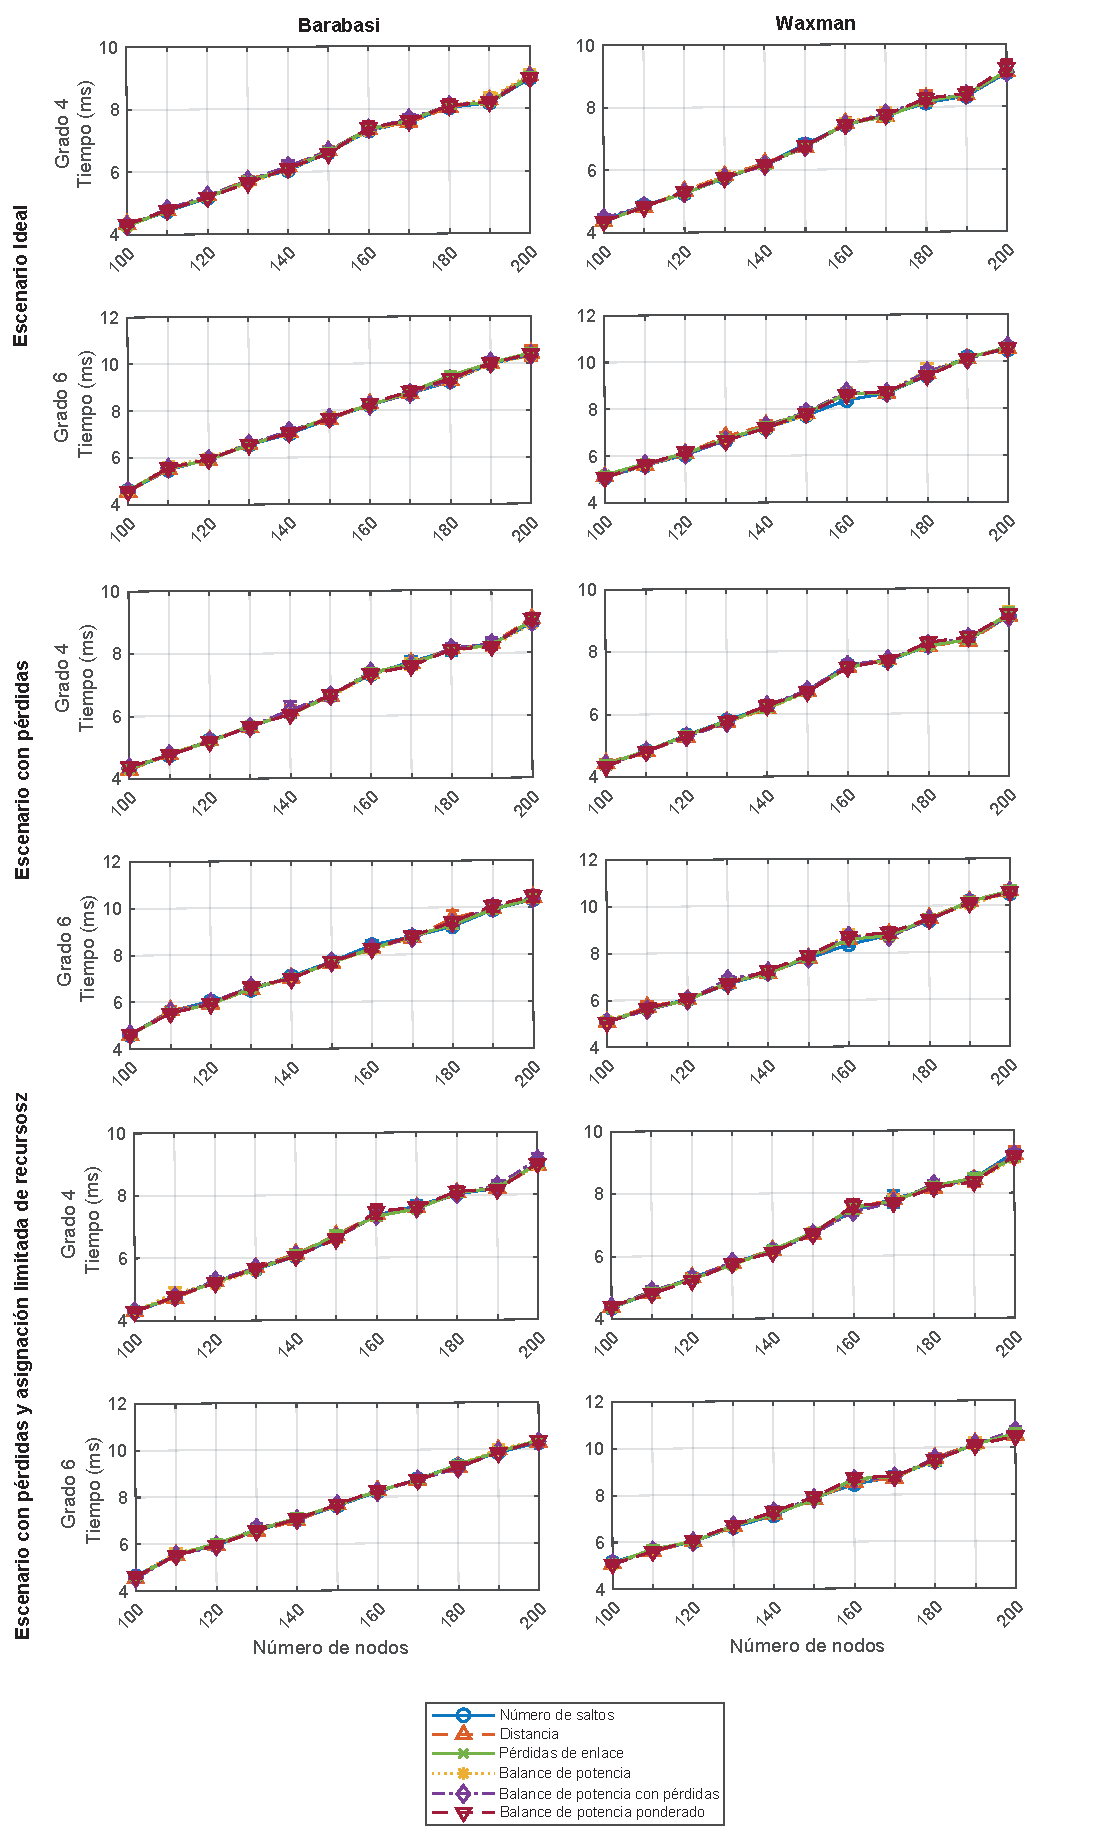
\includegraphics[width=0.85\textwidth]{fig/05_den2ne/den2ne_19.pdf}
    \caption{Tiempo de convergencia de la asignación de etiquetas - Tres escenarios y dos grados de red.}
    \label{fig:f4}
\end{figure}

\begin{figure}[H]
    \centering
    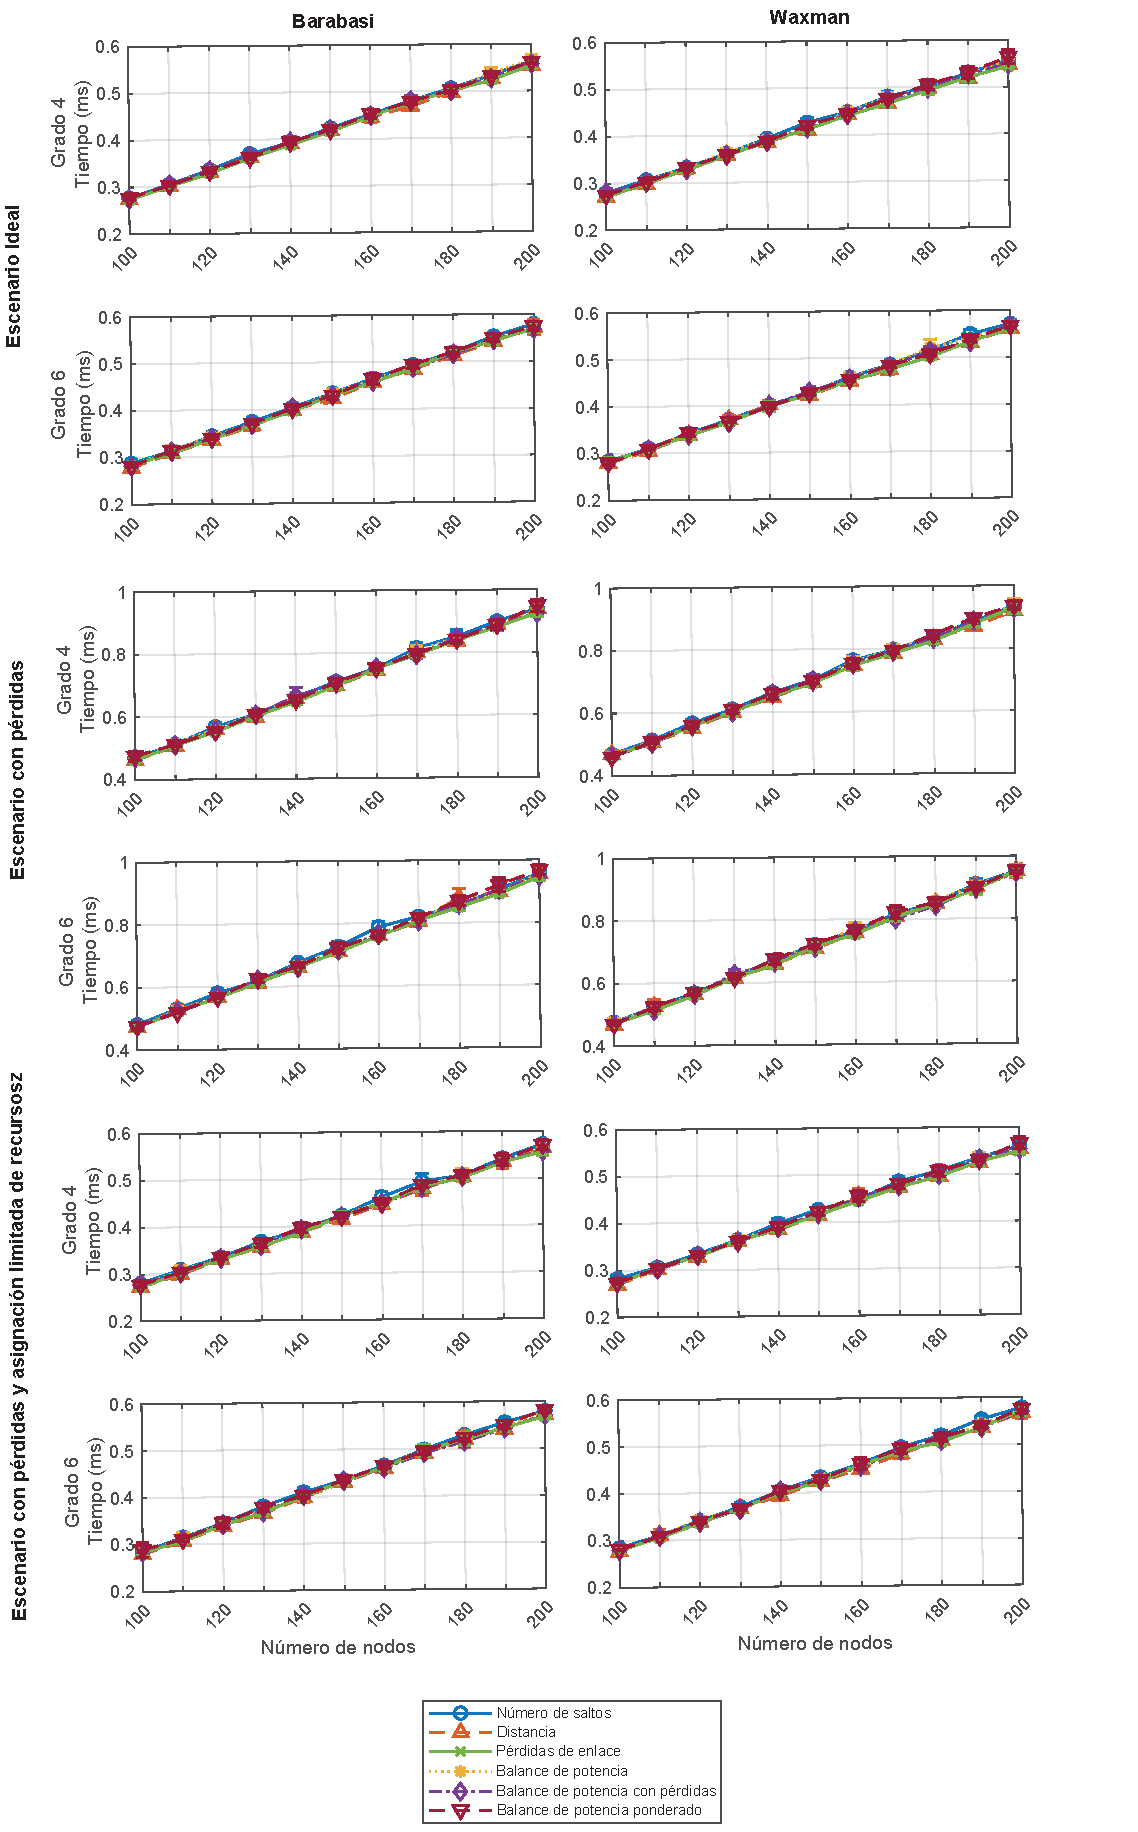
\includegraphics[width=0.85\textwidth]{fig/05_den2ne/den2ne_20.pdf}
    \caption{Tiempo de convergencia del balance de recursos - Tres escenarios y dos grados de red.}
    \label{fig:f3}
\end{figure}

\section{Conclusiones}

En este trabajo se ha presentado \gls{d2e}, un algoritmo para la gestión de recursos en redes densas multi-hop que destaca por su elevada escalabilidad y bajos tiempos de convergencia.\\
\\
El algoritmo descubre los diferentes nodos de la topología y asigna a cada uno de ellos una o varias etiquetas jerárquicas, que representan múltiples rutas hacia el nodo raíz o \textit{gateway}. Posteriormente, redistribuye la carga de trabajo desde los nodos situados en la parte inferior de la jerarquía hasta los niveles superiores. Esta reorganización de recursos puede llevarse a cabo siguiendo distintos criterios: en este trabajo se han evaluado seis como ejemplos representativos, aunque el algoritmo no está limitado a ellos, pudiendo adaptarse fácilmente a otros criterios en función del escenario de aplicación. La evaluación se ha realizado sobre un amplio rango de topologías, con hasta 200 nodos, mostrando tiempos de convergencia reducidos (inferiores a 20 ms) y con un crecimiento lineal. Esta característica resulta especialmente beneficiosa en escenarios con alta movilidad y/o que requieren una mayor fiabilidad. Además, el procedimiento de asignación de etiquetas se ejecuta en solo dos pasos, y cada nodo únicamente necesita almacenar tantas etiquetas como caminos existan hacia el nodo raíz, independientemente del tamaño de la red.\\
\\
Cabe destacar que con \gls{d2e} se sientan las bases para el desarrollo de mecanismos de control, esquemas de encaminamiento basados en etiquetado jerárquico y estrategias de gestión y planificación de recursos en entornos densos y heterogéneos (por ejemplo, \gls{sg}, logística, \textit{edge/fog computing}, entre otros). \gls{d2e} demuestra que es posible combinar asignación jerárquica de rutas, selección de rutas mediante criterios adaptables y una fase de balanceo eficiente con complejidad y requerimientos reducidos, propiedades que resultan críticas en nodos con capacidad limitada. Encajando estas características, directamente con los objetivos de la Tesis.
